%% TODO: coalgebra examples on CPO

\documentclass[letterpaper, 11pt, oneside]{memoir}
\usepackage[english]{babel}
\usepackage[utf8]{inputenc}

% Margins and margin notes.
%% \setlrmargins{3cm}{*}{*}
\setlrmarginsandblock{3cm}{4.5cm}{*}
\setulmarginsandblock{3cm}{3cm}{*}
\setmarginnotes{1cm}{2.5cm}{\onelineskip}
\checkandfixthelayout

% My pagestyle.
\usepackage{calc}

\newlength{\myheadwidth}
\setlength{\myheadwidth}{\textwidth + 3cm}

\makepagestyle{mypagestyle}
\makerunningwidth{mypagestyle}{\textwidth}
\makeheadposition{mypagestyle}{flushleft}{flushleft}{flushleft}{flushleft}

\makeevenhead{mypagestyle}{\leftmark\quad \rightmark}{}{\thepage}
\makeoddhead{mypagestyle}{\leftmark\quad \rightmark}{}{\thepage}

\makeheadrule{mypagestyle}{\textwidth}{1pt}

% Mark setters.
\renewcommand*{\sectionmark}[1]{\markboth{\thesection}{#1}}

% No plain pagestyle.
\aliaspagestyle{plain}{empty}

% Font.
\usepackage{libertine}

% Links and references.
\usepackage{xcolor}
\definecolor{orange}{rgb}{1,0.58,0.06}
\definecolor{blue}{rgb}{0.3,0.77,1}
\definecolor{myred}{rgb}{0.6,0,0}
\usepackage[a4paper,colorlinks,citecolor=blue,linkcolor=orange,urlcolor=orange,pdfpagemode=None]{hyperref}
\renewcommand{\UrlFont}{\ttfamily\scriptsize}

% Color boxes (for notes).
\usepackage{tcolorbox}

% Mathematics.
\usepackage{amsmath, amscd, amssymb, mathrsfs, mathtools, accents, amsfonts, amsthm}

\newtheoremstyle{myteo}{\topsep}{\topsep}
        {}
        {}
        {\bfseries}
        {.}
        {2pt}
        {\thmname{#1}\thmnumber{ #2}\thmnote{ (#3)}}
\theoremstyle{myteo}

\newtheorem{theorem}{Theorem}[section]
\newtheorem{proposition}[theorem]{Proposition}
\newtheorem{lemma}[theorem]{Lemma}
\newtheorem{corollary}[theorem]{Corollary}
\newtheorem{definition}[theorem]{Definition}
\newtheorem{example}[theorem]{Example}
\newtheorem{remark}[theorem]{Remark}
\newtheorem{notation}[theorem]{Notation}

\numberwithin{equation}{section}

% Figures.
\usepackage{caption}
\usepackage{tikz}
\usetikzlibrary{cd}
\usetikzlibrary{fadings}

% Bibliography.
\usepackage[
  backend=biber,
  style=alphabetic,
  sorting=ynt
]{biblatex}
\addbibresource{refs.bib}
\nocite{*}

% My commands.
\newcommand{\marginnote}[1]{\marginpar{\footnotesize #1}}

\DeclareMathOperator*\colim{colim}

\newcommand{\id}{\textsf{id}}
\newcommand{\head}{\textsf{head}}
\newcommand{\tail}{\textsf{tail}}
\newcommand{\body}{\textsf{body}}
\newcommand{\Ord}{\textsf{Ord}}
\newcommand{\alg}{\textsf{Alg}}
\newcommand{\Alg}{\textsf{Alg}}
\newcommand{\Coalg}{\textsf{Coalg}}
\newcommand{\Set}{\textsf{Set}}
\newcommand{\Sub}{\textsf{Sub}}
\newcommand{\Pos}{\textsf{Pos}}
\newcommand{\op}{\text{op}}
\newcommand{\CPO}{\textsf{CPO}}
\newcommand{\MS}{\textsf{MS}}
\newcommand{\N}{\mathbb{N}}
\newcommand{\A}{\mathscr{A}}
\newcommand{\B}{\mathscr{B}}
\newcommand{\D}{\mathscr{D}}
\newcommand{\comma}{,}

\newcommand{\outofcoprod}[2]{{[#1, #2]}}
\newcommand{\intoprod}[2]{{\langle #1, #2\rangle}}

\newcommand{\fundef}[5]{\begin{align*}
    #1\colon\begin{tikzcd}[sep=large]#2\end{tikzcd} &\longrightarrow \begin{tikzcd}[sep=large]#3\end{tikzcd}\\
      \begin{tikzcd}[sep=large]#4\end{tikzcd} &\longmapsto \begin{tikzcd}[sep=large]#5\end{tikzcd}
\end{align*}}

% The document.
\begin{document}

\title{Notes on Initial Algebras and Terminal Coalgebras}
\author{Gabriele Rastello}
\maketitle

\pagestyle{mypagestyle}

\tableofcontents

\chapter{Preliminaries}
\newpage

\section{Limits and colimits}

Through this section let \(\A, \mathscr{D}\) be categories with \(\mathscr{D}\) small.
We recall what limits and colimits are, some significant examples (particularly products and coproducts) and some of their basic properties.
We also introduce some notation.
For detailed proofs see \cite[Chapter 2]{handbook1}.

\begin{definition}
  Given a functor \(F \colon \mathscr{D} \to \A\) a \textbf{cone} \marginnote{cone} on \(F\) is an object \(C \in \A\) and a family of arrows \(\left(\pi_D \colon C \to FD\right)_{D \in \mathscr{D}}\) such that for every arrow \(d \colon D_1 \to D_2\) of \(\mathscr{D}\) we have
  \begin{equation}
    \label{eq:cone}
    Fd \circ \pi_{D_1} = \pi_{D_2}.
  \end{equation}
  The arrows \(\pi_D\) are called \textbf{projections} of the cone, the object \(C\) the \textbf{vertex}.
  \marginnote{projection, vertex}
\end{definition}

\begin{definition}
  Given a functor \(F \colon \mathscr{D} \to \A\) a \textbf{limit} \marginnote{limit} of \(F\) is a cone \((L, (\pi_D)_{D \in \mathscr{D}})\) such that for every other cone \((C, (\rho_D)_{D \in \mathscr{D}})\) there is a unique arrow \(m \colon C \to L\) such that
  \begin{equation*}
    \rho_D = \pi_D \circ m \quad \text{for every \(D \in \mathscr{D}\)}.
  \end{equation*}
\end{definition}

\begin{proposition}
  \label{prop:limit_uniqueness}
  When a functor \(F\) has a limit that limit is unique (up to isomorphism).
\end{proposition}

The following proposition is a way of proving equality of two arrows into a limit.
It is most useful when working in abstract categories where arrows are not (generally) functions.

\begin{proposition}
  \label{prop:arrows_into_limit}
  Let \((L, (\pi_D)_{D \in \mathscr{D}})\) be the limit of \(F\) and consider two arrows \(f,g \colon C \to L\).
  If for every \(D \in \mathscr{D}, \pi_D \circ f = \pi_D \circ g\) then \(f = g\).
\end{proposition}

The definitions of cone and of limit are dualized to yield those of cocone and colimit.

\begin{definition}
  Given a functor \(F \colon \mathscr{D} \to \A\) a \textbf{cocone} \marginnote{cocone} on \(F\) is an object \(C \in \A\) and a family of arrows \(\left(\sigma_D \colon FD \to C \right)_{D \in \mathscr{D}}\) such that for every arrow \(d \colon D_1 \to D_2\) of \(\mathscr{D}\) we have
  \begin{equation}
    \label{eq:cocone}
    \sigma_{D_2} \circ Fd = \sigma_{D_1}.
  \end{equation}
  The arrows \(\sigma_D\) are called \textbf{coprojections} of the cocone.
  \marginnote{coprojection}
\end{definition}

\begin{definition}
  Given a functor \(F \colon \mathscr{D} \to \A\) a \textbf{colimit} \marginnote{colimit} of \(F\) is a cocone \((L, (\sigma_D)_{D \in \mathscr{D}})\) such that for every other cocone \((C, (\tau_D)_{D \in \mathscr{D}})\) there is a unique arrow \(m \colon L \to C\) such that
  \begin{equation*}
    \tau_D = m \circ \sigma_D \quad \text{for every \(D \in \mathscr{D}\)}.
  \end{equation*}
\end{definition}

Propositions \ref{prop:limit_uniqueness} and \ref{prop:arrows_into_limit} are dualized as follows.

\begin{proposition}
  \label{prop:colimit_uniqueness}
  When a functor \(F\) has a colimit that colimit is unique (up to isomorphism).
\end{proposition}

\begin{proposition}
  \label{prop:arrows_from_colimit}
  Let \((L, (\sigma_D)_{D \in \mathscr{D}})\) be the colimit of \(F\) and consider two arrows \(f,g \colon L \to C\).
  If for every \(D \in \mathscr{D}, f \circ \sigma_D =  g \circ \sigma_D\) then \(f = g\).
\end{proposition}

\subsection{Products and coproducts}

We now turn to two particular classes of (co)limits: products and coproducts.
Recall that a discrete category is a category that has no non-identity arrow.

\begin{definition}
  Given a functor \(F \colon \mathscr{D} \to \A\) where \(\mathscr{D}\) is some discrete category a limit of \(F\) is called a \textbf{product} while a colimit a \textbf{coproduct}.
  \marginnote{product, coproduct}
\end{definition}

\begin{notation}
  Notice that to give a functor from a discrete category to \(\A\) is equivalent to picking an element of \(\A\) for every element of \(\mathscr{D}\).
  We thus speak of the ``product of \(A\) and \(B\)'' for \(A, B \in \A\) without explicit reference to any functor.
  Moreover we denote the product of \(A\) and \(B\) in \(\A\), when it exists, by \(A \times B\).
  Similarly we speak of the coproduct of two elements of \(\A\) and denote it by \(A + B\) when it exists.
\end{notation}

\begin{proposition}
  In a category, when the interested (co)products exists, we have that
  \begin{itemize}
  \item[1.] \(A \times B\) is isomorphic to \(B \times A\);
  \item[2.] \(A + B\) is isomorphic to \(B + A\);
  \item[3.] \((A \times B) \times C\) is isomorphic to \(A \times (B \times C)\);
  \item[4.] \((A + B) + C\) is isomorphic to \(A + (B + C)\).
  \end{itemize}
\end{proposition}

In light of this proposition we write \(A \times B \times C\) and \(A + B + C\) with no parenthesis and similarly for any finite number of factors or addenda.

\begin{notation}
  When we take the (co)product of an infinite number of objects of \(\A\) we use the notation \(\prod_{i\in I}A_i\) (for products) and \(\coprod_{i \in I}A_i\) (for coproducts).
  Notice that the order of the factors/addenda does not matter.
\end{notation}

\begin{notation}
  \label{not:brackets}
  Let \((L = \prod_{i\in I}A_i, (\pi_i)_{i \in I})\) be a product in \(\A\).
  Then by Proposition \ref{prop:arrows_into_limit} there is a one-to-one correspondance between arrows \(f \colon C \to L\) and cones \((C, (\rho_i\colon C \to A_i)_{i \in I})\).
  Moreover any collection of arrows \((\rho_i \colon C \to A_i)_{i \in I}\) satisfies condition (\ref{eq:cone}) so it is a cone.
  This means that to give an arrow \(f \colon C \to L\) is equivalent to giving a family of arrows \((\rho_i \colon C \to A_i)_{i \in I}\) so we write
  \begin{equation}
    f = \langle\rho_1, \rho_2, \rho_3, \ldots\rangle;
  \end{equation}
  given a convenient ordering on \(I\).

  By a dual argument we obtain that arrows \(f \colon L \to C\) out of a coproduct \(L = \coprod_{i \in I}A_i\) are in one-to-one correspondence with families of arrows \((\tau_i \colon A_i \to C)\) and write
  \begin{equation}
    f = [\tau_1, \tau_2, \tau_3, \ldots]
  \end{equation}
  for a convenient ordering on \(I\).
\end{notation}

\begin{notation}
  \label{not:product_arrows}
  Let \(A,B,C,D\) be objects of \(\A\) such that \(A \times B, C \times D\) exist and let \(f \colon A \to C, g \colon B \to D\) be arrows.
  With reference to the following diagram we denote \(\langle f \circ \pi_1, g \circ \pi_2\rangle\) by \(f \times g\).
  Dually if \(A + B, C + D\) exist we denote \([\sigma_1 \circ f, \sigma_2 \circ g]\) by \(f + g\).
  \marginnote{\(f \times g\), \(f + g\)}
  \begin{center}
    \begin{tikzcd}[sep = large]
      A \ar[r, "f"]& C \\
      A \times B \ar[u, "\pi_1"] \ar[d, "\pi_2"] \ar[r, dashed, "f \times g"] & C \times D \ar[u] \ar[d]\\
      B \ar[r, "g"]& D
    \end{tikzcd}\quad
    \begin{tikzcd}[sep = large]
      A \ar[d] \ar[r, "f"] & C  \ar[d, "\sigma_1"]\\
      A + B \ar[r, dashed, "f + g"] & C + D\\
      B \ar[u] \ar[r, "g"] & D  \ar[u, "\sigma_2"]
    \end{tikzcd}
  \end{center}
\end{notation}

The next proposition shows how the notation introduced above for products interacts with the composition.
It is most useful for performing calculations; we will use it without explicit reference particularly in the proof of the Primitive Recursion Theorem (see \ref{teo:primitive_recursion}).

\begin{proposition}
  Consider the following diagram.
  \begin{center}
    \begin{tikzcd}[sep = large]
      & & A \ar[r, "g_1"] & D \\
      D \ar[r, "h"] & C \ar[ur, "f_1"] \ar[rd, "f_2"'] \ar[r, "\intoprod{f_1}{f_2}"] & A \times B \ar[u] \ar[d] \ar[r, "g_1 \times g_2"] & D \times E \ar[u] \ar[d]\\
      & & B \ar[r, "g_2"]& E
    \end{tikzcd}\quad
    % \begin{tikzcd}[sep = large]
    %   & & A \\
    %   D \ar[r, "g"] & C \ar[ur, "f_1"] \ar[rd, "f_2"'] \ar[r, "\intoprod{f_1}{f_2}"] & A \times B \ar[u] \ar[d] \\
    %   & & B
    % \end{tikzcd}
  \end{center}
  We have that
  \begin{itemize}
  \item[1.] \((g_1 \times g_2) \circ \intoprod{f_1}{f_2} = \intoprod{g_1 \circ f_1}{g_2 \circ f_2}\);
  \item[2.] \(\intoprod{f_1}{f_2} \circ h = \intoprod{f_1 \circ h}{f_2 \circ h}\).
  \end{itemize}
\end{proposition}

\subsection{Initial and terminal objects}

\begin{definition}
  An \textbf{initial object} \marginnote{initial object} for a category \(\A\) is an object \(0 \in \A\) such that for every other object \(A \in \A\) there is exactly one arrow from \(0\) to \(\A\).
  Dually a \textbf{terminal object} \marginnote{terminal object} for \(\A\) is an object \(1 \in \A\) such that for every other object \(A \in \A\) there is exactly one arrow from \(A\) to \(1\).
\end{definition}

\begin{remark}
  Initial objects, when they exist, are colimits of the functor from the empty category into \(\A\); as such they are all isomorphic and we speak of \emph{the} initial object.
  Dually terminal objects are limits of the functor from the empty category and are unique as well.
\end{remark}

\subsection{(Co)limit-preserving functors}

\begin{definition}
  A functor \(G \colon \A \to \B\) \textbf{preserve limits} \marginnote{limit preservation} if, for every small category \(\D\) and functor \(F \colon \D \to \A\), when the limit of \(F\) exists the limit of \(G \circ F\) is obtained by applying \(G\) to the limit cone.
  That is: if \((L, (\pi_D)_{D \in \D})\) is the limit of \(F\) then \((GL, (G\pi_D)_{D \in \D})\) is the limit of \(G \circ F\).
  As expected \(G\) \marginnote{colimit preservation} is said to preserve colimits when, for every small category \(\D\) and functor \(F \colon \D \to \A\), when the colimit of \(F\) exists then the colimit of \(G \circ F\) is the image through \(G\) of the colimit cocone.
\end{definition}

By restricting the definition above to a specific small category \(\D\) we obtain the notion of a functor that preserves \(\D\)-(co)limits.
We will be interested in functors that preserve \(\omega\)-(co)limits where \(\omega\) is the set of natural numbers with the usual ordering regarded as a category.

\section{Other notations}

\begin{notation}
  When we are working with a category \(\A\) that has enough structure \footnote{i.e. that has all the (co)limits needed for our definition to make sense.} we will often define endofunctors \(F \colon \A \to \A\) by their action on objects only such as
  \begin{equation*}
    FX = X \times X + 1.
  \end{equation*}
  This means that the functor \(F\) sends objects \(A\) to \(A \times A + 1\) (where \(1\) is the terminal object of \(\A\)) and arrows \(f\) to \(f \times f + \id_1\).
\end{notation}

\chapter{Algebras for endofunctors}
\newpage

\section{\(F\)-algebras}

Though this section let \(\mathscr{A}\) be an arbitrary category that we call the \textbf{base category} and \(F \colon \mathscr{A} \to \mathscr{A}\) an endofunctor.

\begin{definition}
  An \textbf{algebra} for \(F\) (or an \textbf{\(F\)-algebra}) is a pair \((A, \alpha)\) where \(A\) is an object of \(\mathscr{A}\) (that we call the \textbf{carrier} or \textbf{base object}) \marginnote{\(F\)-algebra} and \(\alpha\) is an arrow of type \(FA \to A\) (that we call the \textbf{structure} of the algebra).
\end{definition}

As one should expect \(F\)-algebras form a category of their own.

\begin{definition}
  Given \(F\)-algebras \((A, \alpha)\) and \((B, \beta)\) a \textbf{morphism} between them is an arrow \(f: A \to B\) of \(\mathscr{A}\) such that
  \begin{center}
    \begin{tikzcd}[sep=large]
      FA \ar[r, "\alpha"] \ar[d, "Ff"] & A \ar[d, "f"] \\
      FB \ar[r, "\beta"] & B
    \end{tikzcd}
  \end{center}
  commutes.
\end{definition}

\begin{remark}
  Given morphisms of algebras \(f \colon (A, \alpha) \to (B, \beta)\) and \(g \colon (B, \beta) \to (C, \gamma)\) their composition is exactly \(g \circ f\); one can easily check that \(g \circ f\) makes the diagram above commute using that \(f\) and \(g\) are morphisms of \(F\)-algebras and that \(F\) is a functor.
  The identity on an algebra \((A, \alpha)\) is exactly \(\id_A\).
\end{remark}

We denote the category of \(F\)-algebras and morphisms of \(F\)-algebras by \(\alg F\).
\marginnote{\(\alg F\)}

\begin{example}
  \label{ex:prepoly1}
  In \(\Set\) let \(1\) be the terminal object \(\{*\}\) and consider the functor
  \begin{equation*}
    FX = X + 1.
  \end{equation*}
  To give an arrow \(\alpha \colon A + 1 \to A\) is equivalent to giving two functions \(\alpha_0 \colon 1 \to A, \alpha_1 \colon A \to A\); that is \(\alpha = [\alpha_1, \alpha_0]\).
  So an algebra for \(F\) is set \(A\) with a constant \(\alpha_0\) and a unary operation \(\alpha_1\).
  A morphism of \(F\)-algebras is a function \(f\) such that
  \begin{center}
    \begin{tikzcd}[sep=large]
      A + 1 \ar[r, "\outofcoprod{\alpha_1}{\alpha_0}"] \ar[d, "f + \id_1"] & A \ar[d, "f"] \\
      B + 1 \ar[r, "\outofcoprod{\beta_1}{\beta_0}"] & B
    \end{tikzcd}
  \end{center}
  commutes.
  This translates, using Proposition \ref{prop:arrows_from_colimit}, into the following two conditions
  \[f \circ \alpha_1 = \beta_1 \circ f, \quad f \circ \alpha_0 = \beta_0.\]
  Which together give that \(f\) preserves the constant and commutes with the unary operation of the algebras.
\end{example}

\begin{example}
  \label{ex:prepoly2}
  Similarly algebras for the endofuctor \(FX = X \times X + 1\) are sets equipped with a constant and a binary operation.
  Morphisms of such algebras preserve the constant and commute with the operation.
  Indeed if \((A, a, \ast_A)\) and \((B, b, \ast_B)\) are two \(F\)-algebras a morphism \(f \colon A \to B\) is a function such that
  \begin{itemize}
  \item[1.] \(f(a) = b\);
  \item[2.] \(f(x \ast_A y) = f(x) \ast_B f(y)\) for all \(x, y \in A\).
  \end{itemize}
  This is reminiscent of structures such as groups and monoids.
\end{example}

\begin{example}
  \label{ex:prepoly3}
  Let \(\Sigma_1\) be a set; then algebras for \(FX = \Sigma_1 \times X\) are sets with a unary operation for every element \(\sigma \in \Sigma_1\).
  Indeed let \(A\) be an \(F\)-algebra and let \(\alpha \colon \Sigma_1 \times A \to A\) be its structure; for a fixed \(\sigma \in \Sigma_1\) we have that \(\alpha(\sigma, -)\) is a unary operation on \(A\).
  Morphisms of \(F\)-algebras in this case commute with all such unary operations.
\end{example}

Examples \ref{ex:prepoly1}, \ref{ex:prepoly2}, \ref{ex:prepoly3} can be generalized with the introduction of polynomial functors over \(\Set\).
This captures the idea of a \(\Sigma\)-algebra from universal algebra and provides a generalization to other base categories with sufficient structure.

\begin{definition}
  A \textbf{signature} \(\Sigma\) is a collection of sets \((\Sigma_n)_{n < \omega}\) where \(\Sigma_n\) is called the set of \(n\)-ary symbols.
  \marginnote{signature}
  The symbols in \(\Sigma_0\) are also called constant symbols (or symbols for constants).
\end{definition}

\begin{definition}
  \label{def:sigma-algebra}
  Given a signature \(\Sigma\) a \textbf{\(\Sigma\)-algebra} is a set \(A\) together with interpretations for every symbol of \(\Sigma\).
  \marginnote{\(\Sigma\)-algebra}
  That is: to every \(\sigma \in \Sigma_0\) we associate a fixed element of \(A\) and to every \(\sigma \in \Sigma_n\) an \(n\)-ary function on \(A\).
  We denote the interpretation of \(\sigma\) in \(A\) by \(\sigma^A\).

  Given two \(\Sigma\)-algebras \(A\) and \(B\) a \textbf{morphism} of \(\Sigma\)-algebras is a function \(f \colon A \to B\) such that
  \begin{equation}
    \label{eq:sigma_morphism_condition1}
    f\sigma^A = \sigma ^B
  \end{equation}
  for every \(\sigma \in \Sigma_0\) and
  \begin{equation}
    \label{eq:sigma_morphism_condition2}
    f(\sigma^A(x_1, \ldots, x_n)) = \sigma^B(f(x_1), \ldots, f(x_n))
  \end{equation}
  for every \(\sigma \in \Sigma_n\) and \(x_1, \ldots, x_n \in A\).
\end{definition}

We will now observe how \(\Sigma\)-algebras can be realized as algebras for specific endofuctors.
To every signature we associate a \textbf{polynomial functor} \marginnote{polynomial functor} \(H_\Sigma \colon \Set \to \Set\) that operates as follows on objects \(X\) and arrows \(f\).
\begin{align*}
  H_\Sigma X &= \coprod_{n < \omega} \Sigma_n \times X^n \\
  H_\Sigma f &= \coprod_{n < \omega} \id_{\Sigma_n} \times \underbrace{f \times \ldots \times f}_{\text{\(n\) times}}
\end{align*}
Then if \(A\) is a \(\Sigma\)-algebra we can define functions \(\alpha_n \colon \Sigma_n \times A^n \to A\) naturally as
\begin{equation}
  \label{eq:algebra_equivalent_definition}
  \alpha_n(\sigma, x_1, \ldots, x_n) \coloneqq \sigma^A(x_1, \ldots, x_n)
\end{equation}
and then \(\alpha \coloneqq \left[\alpha_0, \alpha_1, \ldots \right]\) makes \(A\) into a \(H_\Sigma\)-algebra.
Conversely if we have a \(H_\Sigma\)-algebra \((A, \alpha)\) we can define an interpretation of every symbol by reading (\ref{eq:algebra_equivalent_definition}) the other way around.

For morphisms consider the following square that we know commutes if \(f\) is a morphism of \(H_\Sigma\)-algebras.
\begin{center}
  \begin{tikzcd}[sep=large]
    \coprod_{n < \omega} \Sigma_n \times A^n \ar[r, "\alpha"] \ar[d, "H_\Sigma f"] & A \ar[d, "f"] \\
    \coprod_{n < \omega} \Sigma_n \times B^n \ar[r, "\beta"] & B
  \end{tikzcd}
\end{center}
Since the diagonal of the square is an arrow out of a coproduct we know from Proposition \ref{prop:arrows_from_colimit} that \(f \circ \alpha\) and \(\beta \circ H_\Sigma f\) are equal when composed with the coprojections of the cocone and this can happen if and only if conditions (\ref{eq:sigma_morphism_condition1}) and (\ref{eq:sigma_morphism_condition2}) hold.\\

%% Give a set \(S\) one can consider the category \(\Set^S\) \marginnote{\(\Set^S\)} of \(S\)-sorted sets where objects are \(S\)-indexed families of sets \((X_s)_{s \in S}\) and arrows from \((X_s)_{s \in S}\) to \((Y_s)_{s \in S}\) are \(S\)-indexed families of functions \((f_s)_{s \in S}\) such that \(f_s \colon X_s \to Y_s\).

%% \begin{definition}
%%   An \textbf{\(S\)-sorted signature} \(\Sigma\) is a set of symbols such that every symbol \(\sigma\) has an arity \(\text{ar}(\sigma)\).
%%   Every arity has the form
%%   \begin{equation*}
%%     s_1 \times \ldots \times s_n \to s
%%   \end{equation*}
%%   where \(s_1, \ldots, s_n, s \in S\).
%%   An \(S\)-sorted algebra for \(\Sigma\) is a set \(A\) together with an interpretation of every symbol in \(\Sigma\).
%%   That is: a symbol \(\sigma\) of arity \(s_1 \times \ldots \times s_n \to s\) is interpreted as a function
%%   \begin{equation*}
%%     \sigma^A \colon A_{s_1} \times \ldots \times A_{s_n} \to A_s.
%%   \end{equation*}
%% \end{definition}

We now turn to continous algebras.

\begin{definition}
  A \textbf{complete partial order} \marginnote{complete partial order} (or a \textbf{CPO}) is a poset \((A, \sqsubseteq)\) in which all \(\omega\)-chains
  \begin{equation*}
    a_1 \sqsubseteq a_2 \sqsubseteq a_3 \sqsubseteq \ldots
  \end{equation*}
  have a join i.e. a least upper bound; we denote it by \(\bigvee_{n < \omega}a_n\).
  A function \(f \colon (A, \sqsubseteq) \to (B, \sqsubseteq)\) is \textbf{continous} \marginnote{continous function} if
  \begin{itemize}
  \item[1.] it is monotone i.e. \(a \sqsubseteq b\) in \(A\) implies \(f(a) \sqsubseteq f(b)\) in \(B\);
  %% \item[2.] if \(\overline{a}\) is the join of \(a_1 \sqsubseteq a_2 \sqsubseteq \ldots\) in \(A\) then \(f(\overline{a})\) is the join of \(f(a_1) \sqsubseteq f(a_2) \sqsubseteq \ldots\) in B.
  \item[2.] given an \(\omega\)-chain \(a_1 \sqsubseteq a_2 \sqsubseteq a_3 \sqsubseteq \ldots\) we have \(f(\bigvee_{n < \omega}a_n) = \bigvee_{n < \omega}f(a_n)\).
  \end{itemize}

  Note that by 1 any chain in \(A\) is preserved by \(f\) and since \(B\) is a CPO it must have a join; condition 2 forces that join to be the image of the join of the original chain under \(f\).
\end{definition}

\begin{remark}
  CPOs and continous functions form a category \(\CPO\).
  In \(\CPO\) (co)products are formed as in \(\Set\) and have, for products, the pointwise order and, for coproducts, each component keeps its own ordering and elements in different components are never comparable.
  Moreover \(\CPO\) has a terminal object \(1\) that is the singleton \(\{*\}\) with the only possible partial order on it.
\end{remark}

\begin{example}
  \label{ex:continous_algebras}
  Consider the functor \(FX = X + 1\) on \(\CPO\).
  Algebras for \(F\) are CPOs with a constant and a continous unary operation.
  Similarly algebras for the functor \(FX = X \times X + 1\) are CPOs with a constant and a continous binary operation.
  The continuity of the operation (which we denote here as \(\ast\)) in this case gives us that if
  \begin{equation*}
    a_0 \sqsubseteq a_1 \sqsubseteq a_2 \sqsubseteq \ldots \quad \text{and} \quad b_0 \sqsubseteq b_1 \sqsubseteq b_2 \sqsubseteq \ldots
  \end{equation*}
  are chains then \((a_0, b_0) \sqsubseteq (a_1, b_1) \sqsubseteq (a_2, b_2) \sqsubseteq \ldots\) is a chain in the product and
  \begin{equation*}
    \bigvee_{n < \omega}a_n \ast \bigvee_{n < \omega}b_n = \bigvee_{n < \omega}a_n \ast b_n.
  \end{equation*}
\end{example}

\begin{example}
  Now let \(FX = X_\bot\) be the functor that adds to a CPO a bottom element (i.e. an element \(\bot\) such that \(\bot \sqsubseteq x\) for every \(x\) in the poset) and that sends a continous function \(f \colon X \to Y\) to \(f_\bot \colon X_\bot \to Y_\bot\) defined as
  \begin{equation*}
    f_\bot(x) = \begin{cases}
      f(x) & \text{if \(x \neq \bot\)}\\
      \bot & \text{if \(x = \bot\)}
    \end{cases}.
  \end{equation*}
  An algebra \((A, \alpha)\) for \(F\) has a unary continous function \(\alpha_1 \colon A \to A\) and a constant \(\alpha_\bot\) such that \(\alpha_\bot \sqsubseteq \alpha(a)\) for every \(a \in A\) by monotony of \(\alpha\).
  Comparing this to Example \ref{ex:continous_algebras} by changing the functor we now have a condition on our constant.
\end{example}

Finally let \(\CPO_\bot\) be the category of CPOs with a bottom element and continous functions that preserve the bottom i.e. such that \(f(\bot) = \bot\).
\marginnote{strict continous function}
We call such functions \textbf{strict continous functions}.

\begin{remark}
  In \(\CPO_\bot\) products work as in \(\CPO\) (the bottom element is naturally the one whose components are all \(\bot\)) but the construction of coproducts must be changed.
  Indeed coproducts in \(\CPO_\bot\) are formed as in \(\CPO\) but the bottoms of all the components are unified into a single element.
  The initial object is still the singleton as it clearly has a bottom.
\end{remark}

\begin{remark}
  Notice that the functor \(FX = X + 1\) on \(\CPO_\bot\) is the identity functor so its algebras are CPOs with a bottom and a strict continous unary operation.
  If we want a constant on top of the unary operation we can consider the functor \(FX = X_\bot + 1_\bot\), \(Ff = f_\bot + \id_{1_\bot}\).
\end{remark}

\section{Initial Algebras}

\begin{definition}
  An \textbf{initial algebra} for an endofunctor \(F\) is an initial object in \(\alg F\).
  \marginnote{initial algebra}
  When an initial algebra exists we denote it by \((\mu F, \iota)\).
\end{definition}

\begin{remark}
  \label{rem:trivial_initial_algebra}
  If \(0\) is the initial object of \(\mathscr{A}\) and \(F\) preserves initial objects then \((0, \id_0)\) is the initial algebra for \(F\).
\end{remark}

We will now look at some non-trivial examples of initial algebras.

\begin{example}
  \label{ex:N}
  Consider the functor \(FX = X + 1\) on \(\Set\).
  The initial algebra for \(F\) is \((\mathbb{N}, \iota)\) where \(\iota = [\iota_1, \iota_0]\) with \(\iota_0 = 0\) and \(\iota_1\) the successor function on the naturals.
  Indeed let \((B, \beta)\) be another algebra with \(\beta = [\beta_1, \beta_0]\) and consider the function \(f \colon \mathbb{N} \to B\) defined as
  \begin{equation}
    \begin{cases}
      f(0) &= \beta_0 \\
      f(n + 1) &= \beta_1(f(n))
    \end{cases}.
  \end{equation}
  This is a morphism of algebras:
  \begin{itemize}
    \item[1.] \(f(0) = \beta_0\);
    \item[2.] \((f \circ \iota_1)(n) = f(n + 1) = (\beta_1 \circ f)(n)\) for all \(n \in \mathbb{N}\) so \(f \circ i_1 = \beta_1 \circ f\);
  \end{itemize}
  and clearly unique because any other morphism must satisfy 1 and 2, thus a simple induction gives us that is must be \(f\).
\end{example}

\begin{example}
  Let \(\mathcal{P}_\textsf{f} \colon \Set \to \Set\) be the finite power-set functor. \marginnote{finite power-set functor}
  This functor sends a set \(X\) to \(\mathcal{P}_\textsf{f}X = \{Z \subseteq X \colon Z\ \text{is finite}\}\) and a function \(f \colon X \to Y\) to the function \(\mathcal{P}_\textsf{f}f\) that sends a finite subset of \(X\) to its (obviously finite) \(f\)-image in \(Y\).
  Let \(V_\omega\) be the set of hereditarily finite sets.
  That is:
  \begin{itemize}
  \item[1.] \(\emptyset \in V_\omega\);
  \item[2.] if \(X_1, \ldots, X_n \in V_\omega\) then \(\{X_1, \ldots, X_n\} \in V_\omega\).
  \end{itemize}
  We will see in Example \ref{ex:finite_powerset_adamek} that \((V_\omega, \id)\) is the initial algebra of \(\mathcal{P}_\textsf{f}\).
\end{example}

\begin{example}
  Let \(\mathscr{A}\) be a category with countable coproducts.
  If \(A \in \mathscr{A}\) we write \(\mathbb{N} \bullet A\) for the coproduct of \(A\) with itself countably many times.
  We shall now consider the functor \(FX = X + A\) for which we prove the initial algebra to be \(\mathbb{N} \bullet A\).

  First we need an algebra structure \(\iota\) on \(\mathbb{N} \bullet A\).
  If \(\textsf{in}_k \colon A \to \mathbb{N} \bullet A\) is the \(k\)-th coprojection then we set
  \begin{equation}
    \iota = [\alpha_1, \textsf{in}_0] \colon (\mathbb{N} \bullet A) + A \to \mathbb{N} \bullet A
  \end{equation}
  where \(\alpha_1\) is obtained from the universal property of the coproduct applied to the cone \((\textsf{in}_k)_{1 < k < \omega}\).
  We thus have that the following triangles commute for every \(k < \omega\).
  \begin{center}
    \begin{tikzcd}[sep = large]
      \mathbb{N} \bullet A \ar[rr, "\alpha_1"] & & \mathbb{N} \bullet A \\
      & A \ar[ul, "\textsf{in}_k"] \ar[ur, "\textsf{in}_{k+1}"']&
    \end{tikzcd}
  \end{center}
  Now let \((B, \beta)\) with \(\beta = [\beta_1, \beta_0]\) be an algebra and \(f\) a morphism from \((\mathbb{N} \bullet A, \iota)\).
  We have that the following square commutes.
  \begin{center}
    \begin{tikzcd}[sep = large]
      \mathbb{N} \bullet A + A \ar[r, "{[\alpha_1, \textsf{in}_0]}"] \ar[d, "f + \id"] & \mathbb{N} \bullet A \ar[d, "f"]\\
      B + A \ar[r, "{[\beta_1, \beta_0]}"] & B
    \end{tikzcd}
  \end{center}
  So any such \(f\) must be such that
  \begin{itemize}
  \item[1.] \(f \circ \textsf{in}_0 = \beta_0\);
  \item[2.] \(f \circ \textsf{in}_{k+1} = f \circ \alpha_1 \circ \textsf{in}_k = \beta_1 \circ f \circ \textsf{in}_k\) for all \(k \in \mathbb{N}\).
  \end{itemize}
  This gives us that \([\beta_0, \beta_1\circ\beta_0, \beta_1\circ\beta_1\circ\beta_0, \ldots]\) is the unique morphism from \((\mathbb{N} \bullet A, \iota)\) to \((B, \beta)\) which proves our claim.
\end{example}

Finally we describe initial algebras for polynomial functors in two equivalent ways: using closed terms and using trees.

\begin{definition}
  Let \(\Sigma\) be a signature.
  The set of \textbf{closed term} for \(\Sigma\) is defined inductively as follows:
  \marginnote{closed term}
  \begin{itemize}
  \item[1.] a constant symbol is a closed term;
  \item[2.] an expression of the form \(\sigma(t_1, \ldots, t_n)\) where \(\sigma \in \Sigma_n\) and \(t_1, \ldots, t_n\) are closed terms is a closed term.
  \end{itemize}
\end{definition}

\begin{remark}
  Let \(\mu H_\Sigma\) be the set of all closed terms; this is naturally a \(\Sigma\)-algebra:
  \begin{itemize}
  \item[1.] if \(\sigma\) is a contant symbol then \(\sigma^{\mu H_\Sigma}\) is \(\sigma\) itself but regarded as a term;
  \item[2.] if \(\sigma\) is an \(n\)-ary symbol then it defines an \(n\)-ary operation on \(\mu H_\Sigma\) that takes terms \(t_1, \ldots, t_n\) to the term \(\sigma(t_1, \ldots, t_n)\).
  \end{itemize}
\end{remark}

\begin{remark}
  \label{rem:ev_function}
  Let \(A\) be a \(\Sigma\)-algebra and \(t\) a closed term.
  We can define an evaluation function \(\textsf{ev} \colon \mu H_\Sigma \to A\) as follows:
  \begin{itemize}
  \item[1.] if \(t\) is a constant symbol \(\sigma\) then \(\textsf{ev}(t) = \sigma^A\);
  \item[2.] if \(t\) is of the form \(\sigma(t_1, \ldots, t_n)\) then \(\textsf{ev}(t) = \sigma^A(\textsf{ev}(t_1), \ldots, \textsf{ev}(t_n))\).
  \end{itemize}
  Clearly \(\textsf{ev}\) is a morphism and moreover it is unique so \(\mu H_\Sigma\) is the initial algebra for \(H_\Sigma\).
\end{remark}

\begin{definition}
  Given a signature \(\Sigma\) a \textbf{\(\Sigma\)-tree} is an ordered tree where every node of \(k\) children is labelled by a \(k\)-ary symbol of \(\Sigma\).
  As an example if \(\sigma_0\) is a constant symbol, \(\sigma_1\) a 2-ary symbol, \(\sigma_2\) a 3-ary symbol and \(\sigma_3\) a 1-ary symbol then the following are valid \(\Sigma\)-trees.
  \begin{equation*}
    \begin{tikzpicture}
      \node (1) at (0, 1){\(\sigma_1\)};
      \node (2) at (-0.75, 0){\(\sigma_0\)};
      \node (3) at (0.75, 0){\(\sigma_0\)};

      \draw[-] (1) -- (2);
      \draw[-] (1) -- (3);
    \end{tikzpicture}\quad\quad
    \begin{tikzpicture}
      \node (1) at (0, 1){\(\sigma_1\)};
      \node (2) at (-0.75, 0){\(\sigma_0\)};
      \node (3) at (0.75, 0){\(\sigma_0\)};
      \node (4) at (0.75, 2){\(\sigma_1\)};
      \node (5) at (1.5, 1){\(\sigma_0\)};
      
      \draw[-] (1) -- (2);
      \draw[-] (1) -- (3);
      \draw[-] (4) -- (5);
      \draw[-] (4) -- (1);
    \end{tikzpicture}\quad\quad
    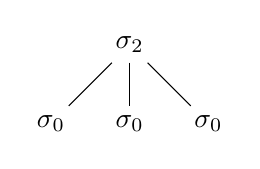
\begin{tikzpicture}
      \node (1) at (0, 1){\(\sigma_2\)};
      \node (2) at (-1, 0){\(\sigma_0\)};
      \node (3) at (0, 0){\(\sigma_0\)};
      \node (4) at (1, 0){\(\sigma_0\)};

      \draw[-] (1) -- (2);
      \draw[-] (1) -- (3);
      \draw[-] (1) -- (4);
    \end{tikzpicture}\quad\quad
    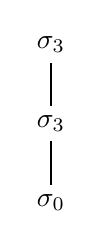
\begin{tikzpicture}
      \node (1) at (0, 0){\(\sigma_0\)};
      \node (2) at (0, 1){\(\sigma_3\)};
      \node (3) at (0, 2){\(\sigma_3\)};

      \draw[-] (1) -- (2) -- (3);
    \end{tikzpicture}
  \end{equation*}
\end{definition}

\begin{remark}
  \label{rem:treetupling}
  Every \(n\)-ary symbol of \(\Sigma\) defines an \(n\)-ary operation on \(\Sigma\)-trees which takes \(n\) trees to the tree obtained by connecting each root to a new node labelled by \(\sigma\), which becomes the root of a new tree.
  We call this operation \textbf{tree-tupling} (below an example of tree-tupling induced by a 3-ary symbol \(\sigma\)).\marginnote{tree-tupling}
  Note that the order of the trees matters.
  \begin{equation*}
    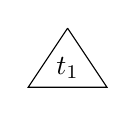
\begin{tikzpicture}
      \node (t) at (0,0){\(t_1\)};
      \draw[-] (0,0.5) -- (.5, -.25) -- (-.5, -.25) -- (0, .5);
    \end{tikzpicture}\quad
    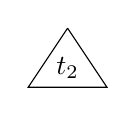
\begin{tikzpicture}
      \node (t) at (0,0){\(t_2\)};
      \draw[-] (0,0.5) -- (.5, -.25) -- (-.5, -.25) -- (0, .5);
    \end{tikzpicture}\quad
    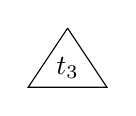
\begin{tikzpicture}
      \node (t) at (0,0){\(t_3\)};
      \draw[-] (0,0.5) -- (.5, -.25) -- (-.5, -.25) -- (0, .5);
    \end{tikzpicture}\quad
    \begin{tikzpicture}
      \node (t) at (0, 3){\(\rightsquigarrow\)};
    \end{tikzpicture}\quad
    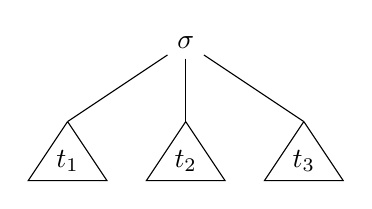
\begin{tikzpicture}
      \node (t1) at (0,0){\(t_1\)};
      \node (t2) at (1.5,0){\(t_2\)};
      \node (t3) at (3,0){\(t_3\)};
      \node (s) at (1.5, 1.5){\(\sigma\)};
      
      \draw[-] (0,0.5) -- (.5, -.25) -- (-.5, -.25) -- (0, .5);
      \draw[-] (1.5,0.5) -- (2, -.25) -- (1, -.25) -- (1.5, .5);
      \draw[-] (3,0.5) -- (3.5, -.25) -- (2.5, -.25) -- (3, .5);

      \draw[-] (s) -- (0,0.5);
      \draw[-] (s) -- (1.5,0.5);
      \draw[-] (s) -- (3,0.5);
    \end{tikzpicture}
  \end{equation*}
\end{remark}

\begin{proposition}
  \label{prop:finite_sigma_trees}
  The initial algebra \(\mu H_\Sigma\) is the algebra of finite \(\Sigma\)-trees with tree-tupling.
\end{proposition}

\begin{proof}
  Let \(T\) be the algebra of finite \(\Sigma\)-trees with tree-tupling; we shall find an isomorphism \(f \colon \mu H_\Sigma \to T\) of algebras.
  Define \(f\) by structural recursion as follows
  \begin{itemize}
  \item[1.] if \(t\) is a constant term \(\sigma\) let \(f(t)\) be the tree formed by a single node labelled by \(\sigma\);
  \item[2.] if \(t\) is a term of the form \(\sigma(t_1, \ldots, t_n)\) let \(f(\sigma)\) be the tree obtained by tree-tupling \(f(t_1), \ldots, f(t_n)\) with the new root labelled by \(\sigma\).
  \end{itemize}
  This function is a morphism by definition and has an inverse, defined similarly by structural recursion, which is again a morphism.
\end{proof}

\begin{example}
  \label{ex:finite_binary_trees}
  By the discussion above the initial algebra for the functor \(FX = X \times X + 1\) on \(\Set\) is the algebra of all finite binary trees.
\end{example}

\begin{example}
  Consider the functor \(FX = B \times X + 1\) on \(\Set\) with \(B \in \Set\).
  Algebras for \(F\) are sets with a constant and \(|B|\) unary operations.
  By the discussion above we know that \(\mu F\) is the algebra of finite trees for the signature \(\Sigma = (\Sigma_0 = \{*\}, \Sigma_1 = B)\) so its elements are ``linear'' trees such as
  \begin{equation*}
    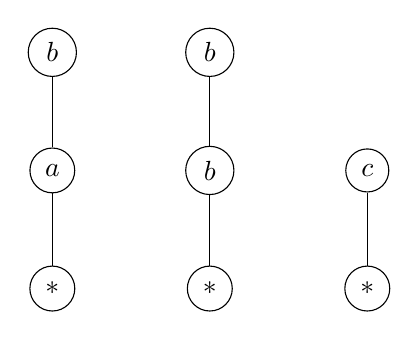
\begin{tikzpicture}
      \path
      (0,0) node[circle, draw](x){\(*\)}
      (0,1.5) node[circle, draw](y){\(a\)}
      (0,3) node[circle, draw](z){\(b\)};
      \draw (x) -- (y) -- (z);

      \path
      (2, 0) node[circle, draw](x){\(*\)}
      (2, 1.5) node[circle, draw](y){\(b\)}
      (2, 3) node[circle, draw](z){\(b\)};
      \draw (x) -- (y) -- (z);

      \path
      (4, 0) node[circle, draw](x){\(*\)}
      (4, 1.5) node[circle, draw](y){\(c\)};
      \draw (x) -- (y);
    \end{tikzpicture}
  \end{equation*}
  with \(a, b, c \in B\).
  We immediately deduce that \(\mu F\) can also be realized as the set of words over \(B\).
\end{example}

\begin{remark}
  Notice the importance of constant symbols.
  Indeed if a polynomial functor on \(\Set\) has no constant then it preserves the initial object 0 so by Remark \ref{rem:trivial_initial_algebra} the initial algebra is trivial.
 Equivalently one can observe that, without constant symbols, the set of closed terms is empty.
\end{remark}

\begin{example}
  Consider \(FX = X_\bot\) on \(\CPO_\bot\).
  Let \(\mathbb{N}^\top\) be the set of the natural numbers with an added topmost element \(\infty\) ordered naturally.
  Notice that \((\mathbb{N}^\top)_\bot\) is isomorphic (as an order) to \(\mathbb{N}^\top\) and consider the successor function \(s \colon (\mathbb{N}^\top)_\bot \to \mathbb{N}^\top\) with \(s(\infty) = \infty\).
  We claim this is the initial algebra for \(F\).

  Let \((A, \alpha)\) be another \(F\)-algebra and \(f \colon (\N^\top, s) \to (A, \alpha)\) a morphism.
  Because \(f\) is an arrow of \(\CPO_\bot\) it must be strict so \(f(0) = \bot\) and because it is a morphism we must have \(f(s(n)) = \alpha(f(n))\); this defines \(f\) inductively on \(\N\).
  Finally we recall that \(f\) must be continous (as an arrow of \(\CPO_\bot\)) so
  \begin{equation*}
    f(\infty) = f \left(\bigvee_{n < \omega} n\right) = \bigvee_{n < \omega}(f(n)).
  \end{equation*}
  This implies that there is really a unique morphism from \((\N^\top, s)\) to \((A, \alpha)\) so \((\N^\top, s)\) is initial.
\end{example}

We conclude this section with the a classic lemma of Lambeck's which gives necessary conditions for functors to have an initial algebra.

\begin{definition}
  A \textbf{fixed point} of an endofunctor \(F\) is an element \(A \in \mathscr{A}\) that is isomorphic to \(FA\).
\end{definition}

\begin{lemma}[Lambeck's Lemma]
  \label{lemma:lambeck}
  An initial algebra for \(F\) is always a fixed point.
\end{lemma}

\begin{proof}
  Let \((\mu F, \iota)\) be the initial algebra of \(F\) so there is a unique morphism
  \begin{equation*}
    f \colon (\mu F, \iota) \to (F(\mu F), F\iota).
  \end{equation*}
  We have that the following diagram commutes
  \begin{equation*}
    \begin{tikzcd}[sep = large]
      F(\mu F) \ar[r, "\iota"] \ar[d, "Ff"] & \mu F \ar[d, "f"]\\
      F(F(\mu F)) \ar[r, "F\iota"] \ar[d, "F\iota"]& F(\mu F) \ar[d, "\iota"]\\
      F(\mu F) \ar[r, "\iota"] & \mu F
    \end{tikzcd}
  \end{equation*}
  so \(\iota \circ f\) is an endomorphism of algebras on the initial algebra; hence it is \(\id_{\mu F}\).
  Now
  \begin{equation*}
    f \circ \iota = F\iota \circ Ff = F(\iota \circ f) = F(\id_{\mu F}) = \id_{F(\mu F)}
  \end{equation*}
  so \(\iota\) is an isomorphism.
  This shows that \(\mu F\) is a fixed point of \(F\).
\end{proof}

\begin{remark}
  We know from Cantor's Theorem that there is no surjection from a given set \(X\) into its power set \(\mathcal{P}X\) so the functor \(\mathcal{P}\) on \(\Set\) has no fixed point hence no initial algebra.
\end{remark}

Lambeck's lemma can be seen as a generalization of the following order-theoretic lemma.

\begin{definition}
  Let \((P, \sqsubseteq)\) be a poset and \(f \colon P \to P\) a monotone function.
  An element \(x \in P\) is a \textbf{pre-fixed point} of \(f\) if \(f(x) \sqsubseteq x\).
\end{definition}

\begin{lemma}
  \label{lemma:order_theory}
  Given a poset \((P, \sqsubseteq)\) and a monotone function \(f \colon P \to P\) let \(A = \{x \in P \colon f(x) \sqsubseteq x\}\) be the set of pre-fixed points of \(f\).
  If \(\overline{a}\) is the meet of \(A\) then \(\overline{a}\) is the least fixed point of \(f\).
\end{lemma}

\begin{proof}
  If \(x \in A\) then \(\overline{a} \sqsubseteq x\) and \(f(\overline{a}) \sqsubseteq f(x) \sqsubseteq x\) follows from monotony of \(f\) and definition of \(A\).
  This shows that \(f(\overline{a})\) is a lower bound for \(A\) so \(f(\overline{a}) \sqsubseteq \overline{a}\).
  Now by applying \(f\) again we obtain \(f(f(\overline{a})) \sqsubseteq f(\overline{a})\) which gives us \(f(\overline{a}) \in A\) and thus \(\overline{a} \sqsubseteq f(\overline{a})\).
  Moreover \(\overline{a}\) must be the least fixed point of \(f\) since all fixed points are pre-fixed points.
\end{proof}

This lemma then gives us the following well-known theorem for free.

\begin{theorem}[Knaster-Tarski Theorem]
  \label{teo:knaster_tarski}
  Let \((L, \sqsubseteq)\) be a complete lattice.
  Then every monotone function of \(L\) has a fixed point.
\end{theorem}

\begin{proof}
  Let \(f\) be a monotone function on \(L\) and \(A\) be the set of pre-fixed points of \(f\).
  It must have a meet \(\overline{a}\) because the lattice is complete so by the Lemma we have a fixed point.
\end{proof}

The generalization of order theoretic results such as Lemma \ref{lemma:order_theory} will be a recurrent theme.
Indeed we can see orders as categories in the usual way, order-preserving functions as functors and pre-fixed points as algebras for these functors.

\section{Recursion and Induction}
\label{sec:recursion_and_induction}

Recursion is a way of defining a function \(f\) on the natural numbers by specifying a value for \(f(0)\) and a way of deriving the value of \(f(n + 1)\) from the value of \(f(n)\).
Recursion, however, can also be used to define functions on (among other things) trees; in this case it is usually called \emph{structural} induction (we have an example of this in Remark \ref{rem:ev_function}).
Here we show how one can use the concept of an initial algebra to provide a general definition of recursion of which the cited examples as particular cases.

\begin{definition}
  Let \(F\) be an endofuctor over \(\A\) with an initial algebra \(\mu F\).
  A morphism \(f \colon \mu F \to A\) of \(\A\) is \textbf{recursively specified} \marginnote{recursively specified morphism} if there exists an algebra structure \(\alpha \colon FA \to A\) on \(A\) that makes \(f\) into an algebra homomorphism (actually the unique algebra homomorphism).
\end{definition}

\begin{example}
  Consider the functor \(FX = X \times X + 1\) on \(\Set\) and let \(T\) be its initial algebra that we know from Example \ref{ex:finite_binary_trees} is the algebra of finite binary trees with tree-tupling.
  Let \(h \colon T \to \mathbb{N}\) be the function that assigns \(0\) to the root-only tree and, given a tree \(t\) obtained by tree-tupling of \(t_1\) and \(t_2\), \(h(t) = 1 + \max\{h(t_1), h(t_2)\}\).
  We now show that \(h\) is recursively specified according to our definition.

  We need an algebra structure on \(\mathbb{N}\) i.e. an arrow \(\alpha \colon \N \times \N + 1 \to \N\).
  Since \(\alpha\) is an arrow out of a coproduct we have \(\alpha = [\alpha_1, \alpha_0]\) so we can let
  \begin{align*}
    \alpha_0 &= 0;\\
    \alpha_1(n, m) &= 1 + \max\{n, m\}.
  \end{align*}
  Indeed if \(\iota_1\) is tree-tupling and \(\iota_0\) is the root-only tree the following square trivially commutes thus \(h\) is recursively specified.
  \begin{equation*}
    \begin{tikzcd}[sep = large]
      T \times T + 1 \ar[r, "\outofcoprod{\iota_1}{\iota_0}"] \ar[d, "h \times h + \id_1"] & T \ar[d, "h"]\\
      \N \times \N + 1 \ar[r, "\outofcoprod{\alpha_1}{\alpha_0}"] & \N
    \end{tikzcd}
  \end{equation*}
\end{example}

The following theorem is a generalization of the classic recursion with parameters theorem.

\begin{theorem}[Primitive Recursion]
  \label{teo:primitive_recursion}
  Assume the base category \(\mathscr{A}\) to have finite products and let \(F\) be an endofunctor with an initial algebra \(\mu F\).
  Then for every \(\alpha \colon F(A \times \mu F) \to A\) there is a unique \(h \colon \mu F \to A\) such that the following square commutes.
  \begin{equation}
    \label{dia:recursion}
    \begin{tikzcd}[sep = large]
      F(\mu F) \ar[r, "\iota"] \ar[d, "F \intoprod{h}{\id_{\mu F}}"] & \mu F \ar[d, "h"] \\
      F(A \times \mu F) \ar[r, "\alpha"] & A
    \end{tikzcd}
  \end{equation}
\end{theorem}

\begin{proof}
  Let \(\pi_1, \pi_2\) be the projections of the product \(A \times \mu F\) and consider the arrow
  \begin{equation*}
    \overline{\alpha} \colon F(A \times \mu F) \xrightarrow{\intoprod{\id_{F(A \times \mu F)}}{F\pi_2}} F(A \times \mu F) \times F(\mu F) \xrightarrow{\alpha \times \iota} A \times \mu F.
  \end{equation*}
  This gives an algebra structure on \(A \times \mu F\) so let \(\overline{h} \colon \mu F \to A \times \mu F\) be the unique algebra homomorphism given by the initiality of \(\mu F\).
  \begin{equation}
    \label{dia:recursion2}
    \begin{tikzcd}[row sep = large, column sep = 6 em]
      F(\mu F) \ar[drr, phantom, "\scriptstyle (1)"] \ar[d, "F\overline{h}"] \ar[rr, "\iota"] & & \mu F \ar[d, "\overline{h}"] \\
      F(A \times \mu F) \ar[r, "\intoprod{\id_{F(A \times \mu F)}}{F\pi_2}"] \ar[drr, phantom, "\scriptstyle (3)", very near start] \ar[d, "F\pi_2"] & F(A \times \mu F) \times F(\mu F) \ar[r, "\alpha \times \iota"] \ar[dl, "\pi_2"] \ar[dr, phantom, "\scriptstyle (2)"] & A \times \mu F \ar[d, "\pi_2"] \\
      F(\mu F) \ar[rr, "\iota"] & & \mu F
    \end{tikzcd}
  \end{equation}
  The outer square in (\ref{dia:recursion2}) commutes because (1), (2) and (3) do.
  Indeed (1) commutes because \(\overline{h}\) is an algebra homomorphism, (2) by Notation \ref{not:product_arrows} and (3) because of Notation \ref{not:brackets}.
  By functoriality of \(F\) we then have that \(\pi_2 \circ \overline{h}\) is an endomorphism on the initial algebra thus \(\pi_2 \circ \overline{h} = \id_{\mu F}\).

  Now set \(h \coloneqq \pi_1 \circ \overline{h}\) so \(\overline{h} = \intoprod{h}{\id_{\mu F}}\).
  Extending (1) by \(\pi_1\) we obtain the following diagram that we know commutes.
  \begin{equation*}
    \begin{tikzcd}[row sep = large, column sep = 6 em]
      F(\mu F) \ar[rr, "\iota"] \ar[d, "F\overline{h} = F\intoprod{h}{\id_{\mu F}}"]& & \mu F \ar[d, "\overline{h}"] \ar[dr, "h"] & \\
      F(A \times \mu F) \ar[r, "\intoprod{\id_{F(A \times \mu F)}}{F\pi_2}"] & F(A \times \mu F) \ar[r, "\alpha \times \iota"] \times F(\mu F) & A \times \mu F \ar[r, "\pi_1"] & A
    \end{tikzcd}
  \end{equation*}
  But notice that
  \begin{equation*}
    \pi_1 \circ (\alpha \times \iota) \circ \intoprod{\id_{F(A \times \mu F)}}{F\pi_2} = \pi_1 \circ \intoprod{\alpha}{\iota \circ F\pi_2} = \alpha.
  \end{equation*}
  so we have (\ref{dia:recursion}).

  To prove uniqueness consider \(h \colon \mu F \to A\) homomorphism of algebras such that (\ref{dia:recursion}) commutes.
  We claim that \(\overline{h} = \intoprod{h}{\id_{\mu F}}\) so that \(h = \pi_1 \circ \overline{h}\); thus uniqueness.
  In order to do it we show that \(\intoprod{h}{\id_{\mu F}}\) is an algebra homomorphism and conclude it must be \(\overline{h}\) by initiality of \(\mu F\).
  Indeed we have
  \begin{align*}
    \pi_1 \circ (\alpha \times \iota) \circ \intoprod{\id_{F(A \times \mu F)}}{F\pi_2} \circ F\intoprod{h}{\id_{\mu F}}
    &= \alpha \circ \id_{F(A \times \mu F)} \circ F\intoprod{h}{\id_{\mu F}} \\
    &= h \circ \iota\\
    &= \pi_1 \circ \intoprod{h}{\id_{\mu F}} \circ \iota;\\
    &\\
    \pi_2 \circ (\alpha \times \iota) \circ \intoprod{\id_{F(A \times \mu F)}}{F\pi_2} \circ F\intoprod{h}{\id_{\mu F}}
    &= \iota \circ F\pi_2 \circ F\intoprod{h}{\id_{\mu F}}\\
    &= \iota \circ F(\pi_2 \circ \intoprod{h}{\id_{\mu F}})\\
    &= \iota \circ F\id_{\mu F}\\
    &= \iota \circ \id_{F(\mu F)}\\
    &= \iota\\
    &= \pi_2 \circ \intoprod{h}{\id_{\mu F}} \circ \iota;
  \end{align*}
  so we conclude by Proposition \ref{prop:arrows_into_limit}.
\end{proof}

Recall the classic recursion with parametes theorem.
We shall prove it using Theorem \ref{teo:primitive_recursion}; for a classical proof see \cite[Theorem 18.1]{andrettaelements}.

\begin{theorem}[Recursion with parameters]
  Let \(A\) be a set, \(a \in A\) and \(f \colon A \times \N \to A\) be a function.
  Then there is a function \(g \colon \N \to A\) such that
  \begin{equation*}
    \begin{cases}
      g(0) = a \\
      g(n + 1) = f(g(n), n)
    \end{cases}.
  \end{equation*}
\end{theorem}

\begin{proof}
  Consider the functor \(FX = X + 1\) on \(\Set\) and form the arrow
  \begin{equation*}
    \alpha \colon F(A \times \mu F) = A \times \N + 1 \xrightarrow{\outofcoprod{f}{a}} A
  \end{equation*}
  where we abuse notation and let \(a : 1 \to A\) be the function that picks \(a \in A\).
  Now by Theorem \ref{teo:primitive_recursion} there is a function \(g \colon \N \to A\) such that (\ref{dia:recursion}) commutes.
  This gives us the diagram
  \begin{equation}
    \begin{tikzcd}[sep = large]
      \N + 1 \ar[r, "\outofcoprod{\iota_1}{\iota_0}"] \ar[d, "\intoprod{g}{\id_\N} + \id_1"] & \N \ar[d, "g"]\\
      A \times \N + 1 \ar[r, "\outofcoprod{f}{a}"] & A
    \end{tikzcd}
  \end{equation}
  that yields the conditions
  \begin{enumerate}
  \item[1.] \(g \circ \iota_0 = a \circ \id_1\);
  \item[2.] \(g \circ \iota_1 = f \circ \intoprod{g}{\id_\N}\).
  \end{enumerate}
  Now 1 gives us \(g(0) = a\) and 2 that
  \begin{equation*}
    g(n + 1) = (g \circ \iota_1)(n) = (f \circ \intoprod{g}{\id_\N})(n) = f(g(n), n) \quad \text{for all \(n < \omega\).}
  \end{equation*}
  So \(g\) has the required properties.
\end{proof}

The induction principle, that if a subset of \(\N\) contains \(0\) and is closed under the successor operation then it is \(\N\), can also be generalized to the more general setting of \(F\)-algebras.
Recall that a subobject in a category is represented by a monomorphism.
We call subalgebras subobjects in \(\alg F\).

\begin{theorem}[Induction Principle]
  \label{th:induction_principle}
  Let \(F\) be an endofunctor and \(\mu F\) its initial algebra.
  Then every \(m \colon (B, \beta) \to (\mu F, \iota)\) monic is an isomorphism.
\end{theorem}

\begin{proof}
  By initiality there is a unique homomorphism of \(F\)-algebras \(h \colon (\mu F, \iota) \to (B, \beta)\).
  Now \(m \circ h\) is an endomorphism of the initial object of \(\alg F\) so \(m \circ h = \id_{\mu F}\), but notice that we have \(m\) monic and split-epi thus an isomorphism.
\end{proof}

\chapter{Initial algebras from finitary iteration}
\newpage

\section{Adámek's Theorem}

We begin this section by recalling Kleene's Fixed Point Theorem and its proof with the goal of generalizing it to the categorical setting.

\begin{theorem}[Kleene's Fixed Point Theorem]
  \label{teo:kleene}
  Let \(A\) be a CPO with bottom \(\bot\); then every continous function \(F \colon A \to A\) has a least fixed point \(\mu F = \sup_{n < \omega}F^n(\bot)\)\footnote{We write \(F^n\) for \(\underbrace{F \ldots F}_{n \text{ times}}\) and \(F^0\) is the identity function. We use a similar notation for functors.}.
\end{theorem}

\begin{proof}
  Consider the \(\omega\)-chain \(\bot \leq F(\bot) \leq F^2(\bot) \leq \ldots\) and let \(\mu F\) be its join.
  By continuity \(F(\mu F) = \bigvee_{n < \omega}F(F^n(\bot))\) but we know that \(\bigvee_{n < \omega}F^n(\bot) = \bigvee_{n < \omega}F^{n+1}(\bot)\) so \(\mu F = F(\mu F)\), a fixed point.

  Now let \(F(x) \leq x\) be a pre-fixed point.
  As \(\bot \leq x\) we have \(F(\bot) \leq F(x) \leq x\) and by induction we obtain that \(F^n(\bot) \leq x\) for all \(n < \omega\).
  But this shows that \(x\) is an upper bound so \(\mu F \leq x\) by definition and, finally, \(\mu F\) must be the least fixed point because it is less than any pre-fixed point and fixed points are trivially pre-fixed points.
\end{proof}

Unsurprisingly we shall replace CPOs with bottom by categories with an initial obejct and endofunctions by endofunctors.
The \(\omega\)-chain used in the proof of Theorem \ref{teo:kleene} becomes a diagram and the continuity condition become a colimit-preservation one.

\begin{definition}
  The \textbf{initial-algebra \(\omega\)-chain}\marginnote{initial-algebra \(\omega\)-chain} of an endofunctor \(F\) is the diagram
  \begin{equation}
    \label{dia:initial_chain}
    \begin{tikzcd}[sep = large]
      0 \ar[r, "!"] & F0 \ar[r, "F!"] & F^20 \ar[r, "F^2!"] & F^30 \ar[r, "F^3!"] & \cdots
    \end{tikzcd}
  \end{equation}
  where we denote by \(!\) the unique arrow out of the initial object.
  This diagram can be realized as a functor from \(\omega\) regarded as a category.
\end{definition}

\begin{remark}
  \label{rem:induced_cocone}
  Let \((A, \alpha)\) be an \(F\)-algebra.
  Then it induces a canonical cocone \((\alpha_n \colon F^n0 \to A)_{n < \omega}\) on (\ref{dia:initial_chain}) by
  \begin{align*}
    \alpha_0 &=\ ! \\
    \alpha_{n+1} &= FF^n0 \xrightarrow{F\alpha_n} FA \xrightarrow{\alpha} A.
  \end{align*}
  To check that the \(\alpha_n\)'s are a cocone we prove \(\alpha_n = \alpha_{n+1} \circ F^n!\) by induction on \(n\).
  When \(n = 0\) the condition becomes \(! = \alpha_1 \circ !\) which is true because both sides are arrows out of the initial object.
  Now suppose the condition holds for \(n - 1\):
  \begin{align*}
    \alpha_{n+1} \circ F^n! &= \alpha \circ F\alpha_n \circ F^k! && \text{definition of \(\alpha_{n+1}\)}\\
    &= \alpha \circ F(\alpha_n \circ F^{n-1}!) && \text{functoriality of \(F\)}\\
    &= \alpha \circ F\alpha_{n-1} && \text{inductive hypothesis}\\
    &= \alpha_n && \text{definition of \(\alpha_n\)}.
  \end{align*}
\end{remark}

\begin{remark}
  If we apply \(F\) to the inital-algebra \(\omega\)-chain we obtain
  \begin{equation}
    \label{dia:initial_chain_F}
    \begin{tikzcd}[sep = large]
      F0 \ar[r, "F!"] & F^20 \ar[r, "F^2!"] & F^30 \ar[r, "F^3!"] & \cdots
    \end{tikzcd}.
  \end{equation}
  This \(\omega\)-chain has the same colimit as the original one.
  Indeed since the first element of (\ref{dia:initial_chain}) is the initial object there is an obvious one-to-one correspondence between cocones on (\ref{dia:initial_chain}) and cocones on the new chain above; and the same factorization morphisms work.
\end{remark}

We are ready to state and prove the main theorem of this chapter.

\begin{theorem}[Adámek]
  \label{teo:adamek}
  Let \(\A\) be a category with an initial object \(0\) and colimits of \(\omega\)-chains and \(F\) an endofunctor that preserves \(\omega\)-colimits.
  Then \(F\) has an initial algebra \(\mu F = \colim_{n < \omega}F^n0\).
\end{theorem}

\begin{proof}
  Let \((\mu F, (c_n \colon F^n0 \to \mu F)_{n < \omega})\) be the colimit of the initial-algebra \(\omega\)-chain.
  Since \(F\) preserves \(\omega\)-colimits we have that \((F(\mu F), (Fc_n \colon F^{n+1} \to F(\mu F))_{n < \omega})\) is the colimit of (\ref{dia:initial_chain_F}) but \((c_{n+1} \colon F^{n+1}0 \to \mu F)_{n < \omega}\) is a cocone on (\ref{dia:initial_chain_F}) so there is a unique arrow \(\iota\) from \(F(\mu F)\) to \(\mu F\) such that
  \begin{equation}
    \label{eq:iota}
    \iota \circ Fc_n = c_{n + 1} \quad \text{for all \(n < \omega\).}
  \end{equation}
  This gives an \(F\)-algebra structure to \(\mu F\) that we now check is initial.

  Let \((A, \alpha)\) be a generic \(F\)-algebra.
  We have the induced cocone \((\alpha_n \colon F^n0 \to \mu F)_{n < \omega}\) as in Remark \ref{rem:induced_cocone} and this gives a unique arrow \(h \colon \mu F \to A\) such that \(h \circ c_n = \alpha_n\) for \(n < \omega\).
  We shall now prove that \(h\) is a morphism of \(F\)-algebras and that it is unique.

  To prove that \( h \circ \iota = \alpha \circ Fh\) we check that both arrows are factorization morphisms for the cocone \((\alpha_{n + 1} \colon F^{n+1}0 \to A)_{n < \omega}\).
  In practice we shall check that
  \begin{equation*}
    h \circ \iota \circ Fc_n = \alpha_{n + 1} = \alpha \circ Fh \circ Fc_n
  \end{equation*}
  for all \(n < \omega\).
  For the first equality notice that \(h \circ \iota \circ Fc_n = h \circ c_{n+1} = \alpha_{n+1}\).
  For the second equality consider the following diagram
  \begin{equation*}
    \begin{tikzcd}[sep = large]
      F^{n+1}0 \ar[r, "\alpha_{n+1}"] \ar[d, "Fc_n"'] \ar[dr, "F\alpha_n"] & A \\
      F(\mu F) \ar[r, "Fh"] & FA \ar[u, "\alpha"']
    \end{tikzcd}.
  \end{equation*}
  The upper-right triangle commutes by definition of \(\alpha_{n + 1}\) (see Remark \ref{rem:induced_cocone}).
  The lower-left triangle commute because \(h\) is the factorization arrow and by functoriality of \(F\).
  Then, as the whole square commutes, \(\alpha \circ Fh \circ Fc_n = \alpha_{n+1}\).
  This proves that \(h \colon \mu F \to A\) is a homomorphism of \(F\)-algebras.

  To prove uniqueness suppose there is an arrow \(k \colon \mu F \to A\) such that it is also an \(F\)-algebra homomorphism i.e. \(k \circ \iota = \alpha \circ Fk\).
  We will show that \(k \circ c_n = \alpha_n\) for all \(n < \omega\) and conclude by uniqueness of \(h\).
  Working by induction, if \(n = 0\) then \(k \circ c_0 = \alpha_0\) is trivial because both arrows are out of the initial object.
  Now suppose that \(k \circ c_n = \alpha_n\):
  \begin{align*}
    k \circ c_{n+1} &= k \circ \iota \circ Fc_n && \text{(\ref{eq:iota})}\\
    &= \alpha \circ Fk \circ Fc_n && \text{\(k\) homomorphism}\\
    &= \alpha \circ F(k \circ c_n) && \text{\(F\) functor}\\
    &= \alpha \circ F\alpha_n && \text{inductive hypothesis}\\
    &= \alpha_{n+1} && \text{definition of \(\alpha_{n+1}\)}.\\
  \end{align*}
  This concludes the proof.
\end{proof}

\begin{remark}
  Looking at the proof of Theorem \ref{teo:adamek} we notice that it isn't really necessary for \(\A\) to have colimits of \emph{all} \(\omega\)-chains or for \(F\) to preserve \emph{all} of them as we care for these properties only when applied to the initial-algebra \(\omega\)-chain.
  However in practice it may be more convenient to check the general properties rather than the particular case.
\end{remark}

We will now look at some examples of functors to which one can apply Adámek's Theorem.
We urge the reader to notice that the Theorem does not only guarantee the existence of an initial algebra, but also that such algebra is a colimit.
By looking at the diagram in question (the initial-algebra \(\omega\)-chain) we can often build an intuition of what the initial algebra is ``internally''.

\begin{remark}
  \label{rem:omega_preservation}
  We shall prove that in a category \(\A\) with binary coproducts, a terminal object \(1\) and colimits of \(\omega\)-chains, the functor \(FX = X + 1\) preserves colimits of \(\omega\)-chains.\\

  Consider an \(\omega\)-chain
  \begin{equation}
    \label{eq:om_chain}
    \begin{tikzcd}[sep = large]
      A_0 \ar[r, "a_0"] & A_1 \ar[r, "a_1"] & A_2 \ar[r, "a_2"] & A_3 \ar[r, "a_3"] & \cdots
    \end{tikzcd}
  \end{equation}
  and let \((A, \alpha_i:A_i \to A)_{i < \omega}\) be its colimit.
  We want to prove that \((A + 1, \alpha_i + \id_1)_{i<\omega}\) is the colimit of
  \begin{equation}
    \label{eq:om_chain2}
    \begin{tikzcd}[sep = large]
      A_0 + 1 \ar[r, "a_0 + \id_1"] & A_1 +1 \ar[r, "a_1 + \id_1"] & A_2 + 1 \ar[r, "a_2 + \id_1"] & A_3 + 1 \ar[r, "a_3 + \id_1"] & \cdots
    \end{tikzcd}.
  \end{equation}
  By functoriality of \(F\) we have immediately that it is a cocone on (\ref{eq:om_chain2}) so we only need to show it is universal.
  Let \((B, \beta_i: A_i + 1 \to B)_{i<\omega}\) be a cocone on (\ref{eq:om_chain2}) and note that for all \(i < \omega, \beta_i = [\beta_i^1, \beta_i^2]\) with \(\beta_i^1:A_i \to B\) and \(\beta_i^2: 1 \to B\).
  By composition with the coprojections of the \(A_i + 1\)'s we obtain that
  \begin{itemize}
  \item[1.] \((B, \beta_i^1)_{i<\omega}\) is a cocone on (\ref{eq:om_chain});
  \item[2.] \((B, \beta_i^2)_{i<\omega}\) is a cocone on
    \begin{equation}
      \label{eq:om_chain3}
      \begin{tikzcd}[sep = large]
        1 \ar[r, "\id_1"] & 1 \ar[r, "\id_1"] & 1 \ar[r, "\id_1"] & 1 \ar[r, "\id_1"] & \cdots
      \end{tikzcd}.
    \end{equation}
  \end{itemize}
  Now (\ref{eq:om_chain}) has colimit \((A, \alpha_i)_{i<\omega}\) and (\ref{eq:om_chain3}) has colimit \((1, \gamma_i = \id_1)_{i<\omega}\) so we obtain unique arrows \(m^1 : A \to B \) and \(m^2:1 \to B\) such that
  \begin{equation*}
    m^1 \circ \alpha_i = \beta_i^1 \quad \text{and} \quad m^2 \circ \id_1 = \beta_i^2 \quad \text{for all \(i<\omega\)}.
  \end{equation*}
  Finally we set \(m = [m^1, m^2]\) and this is a factorization arrow for \((B, \beta_i)_{i<\omega}\) as the following calculation shows
  \begin{align*}
    m \circ (\alpha_i + \id_1) &= [m^1, m^2] \circ (\alpha_i + \id_1)\\
                      &= [m^1 \circ \alpha_i, m^2 \circ \id_1]\\
                      &= [\beta_i^1, \beta_i^2]\\
                      &= \beta_i.
  \end{align*}
  We only need to show that such \(m:A + 1 \to B\) is unique.
  Let \(n: A + 1 \to B\) be such that \(n \circ (\alpha_i + \id_1) = \beta_i\) for all \(i<\omega\).
  Since \(n\) is an arrow out of a coproduct we have \(n = [n^1, n^2]\) with \(n^1:A \to B, n^2:1 \to B\).
  Then from the factorization condition we obtain \([n^1 \circ \alpha_i, n^2 \circ \id_1] = [\beta_i^1, \beta_i^2]\) and, by composing with the coprojects, \(n^1 \circ \alpha_i = \beta_i^1\) and \(n^2 \circ \id_1 = \beta_i^2\) for all \(i < \omega\).
  But now we must have \(n^1 = m^1\) and \(n^2 = m^2\) because \(m^1, m^2\) are unique.
  Finally \(n = m\) and \(F\) preserves colimits of \(\omega\)-chains.\\

  By a similar argument one can show that all polynomial functors preserve colimits of \(\omega\)-chains.
\end{remark}

\begin{example}
  In a category with binary coproducts and an initial object 1 the initial algebra for \(FX = X + 1\), if it exists, is called the \textbf{natural numbers object} (or \textbf{NNO}) \marginnote{natural numbers object} of the category.
  Notice that a NNO, being an initial algebra, is unique so the use of ``the'' is justified.
  Explicitly a NNO is a pair \((N, \iota:N+1 \to N)\) such that for every other pair \((A, \alpha : A+1 \to A)\) there is a unique \(h:N\to A\) such that
  \begin{equation*}
    \begin{tikzcd}[sep = large]
      N + 1 \ar[r, "\iota"] \ar[d, "h + \id_1"] & N \ar[d, "h"]\\
      A + 1 \ar[r, "\alpha"] & A
    \end{tikzcd}
  \end{equation*}
  commutes.
  By Adámek's Theorem the NNO is the colimit of the \(\omega\)-chain
  \begin{equation*}
    \begin{tikzcd}[sep = large]
      0 \ar[r] & 1 \ar[r] & 1 + 1 \ar[r] & 1 + 1 + 1 \ar[r] & \cdots
    \end{tikzcd}.
  \end{equation*}
  So if \(\A = \Set\) the chain above becomes the sequence of natural numbers, where each \(n \in \N\) is regarded as the set \(\{0, \ldots, n-1\}\), and \(N\) will thus be exactly \(\N\); hence the name ``natural numbers object''. 
\end{example}

\begin{example}
  On \(\Pos\), the category of partially ordered sets and order-preserving functions, consider the functor \(FX = X_\bot\).
  Its initial-algebra \(\omega\)-chain is
  \begin{equation*}
    \begin{tikzpicture}[every node/.style={outer sep=0.5cm}]
      \node (1) at (0, 0){\(\emptyset\)};
      \node (2) at (2, 0){\(\bot\)};
      \node (3) at (4, 0.5){\(\bullet\)};
      \node (4) at (4, -0.5){\(\bot\)};
      \node (5) at (6, 1){\(\bullet\)};
      \node (6) at (6, 0){\(\bullet\)};
      \node (7) at (6, -1){\(\bot\)};
      \node (8) at (8, 0){\(\cdots\)};
      \node (9) at (4, 0){};

      \draw[-] (3) -- (4);
      \draw[-] (5) -- (6) -- (7);

      \draw[->] (0.35, 0) to (1.65, 0);
      \draw[->] (2.35, 0) to (3.65, 0);
      \draw[->] (4.35, 0) to (5.65, 0);
      \draw[->] (6.35, 0) to (7.65, 0);
      
    \end{tikzpicture}
  \end{equation*}
  So the \(n\)-th element of the \(\omega\)-chain can be thought of as the set \(n = \{0, \ldots, n-1\}\) with the natural order upon it while the connecting morphisms are inclusions.
  The colimit is \(\N\) with the standard ordering.
\end{example}

\begin{definition}
  A function \(f : M \to M'\) between metric spaces \((M, d_M), (M', d_{M'})\) is \textbf{non-expanding} \marginnote{non-expanding map} if \(d_{M'}(f(x), f(y)) \leq d_M(x,y)\) for all \(x,y \in M\).
  A metric space \((M, d_M)\) is \(1\)-bounded if \(d_M(x, y) \leq 1\) for all \(x,y \in M\).
  We denote by \(\MS\) the category of \(1\)-bounded metric spaces and non-expanding maps \marginnote{\(\MS\)}.
\end{definition}

\begin{remark}
  Coproducts in \(\MS\) are disjoint unions where each summand retains its metric and points in different summands have distance \(1\).
  The product of \(M, M' \in \MS\) is the cartesian product \(M \times M'\) endowed with the maximum metric
  \begin{equation*}
    d_{M \times M'}((x, x'), (y, y')) = \max\{d_M(x, y), d_{M'}(x', y')\}.
  \end{equation*}
  Moreover \(\MS\) has a terminal object \(1 = \{*\}\) i.e. the singleton with its unique metric.
\end{remark}

\begin{example}
  We can now consider \(FX = X + 1\) on \(\MS\).
  The objects of the initial-algebra \(\omega\)-chain are again the natural numbers \(n = \{0, \ldots, n-1\}\), but this time regarded as discrete spaces (that is: spaces where all points have distance \(1\)) and the connecting arrows are the inclusions.
  Thus the colimit, and initial algebra of \(F\), is \(\N\) endowed with the discrete metric.

  Now consider the functor \(FX = \frac{1}{2}X + 1\) where we denote by \(\frac{1}{2}X\) the space obtained by scaling the metric of \(X\) by a factor of \(\frac{1}{2}\).
  This functor preserves colimits of \(\omega\)-chains by Remark \ref{rem:omega_preservation}, mutatis mutandis.
  Its initial-algebra \(\omega\)-chain in the following sequence of spaces
  \begin{equation*}
    \begin{tikzpicture}[every node/.style={outer sep=0.5cm}]
      \node (1) at (0, 0){\(\emptyset\)};
    \end{tikzpicture},\quad
    \begin{tikzpicture}[every node/.style={outer sep=0.5cm}]
      \node (1) at (0, 0){\(0\)};
    \end{tikzpicture},\quad
    \begin{tikzpicture}
      \node (1) at (0, 0){\(0\)};
      \node (2) at (2, 0){\(1\)};
      \node (3) at (1, 0)[above]{\small 1};
      \draw[dashed] (1) to (2);
    \end{tikzpicture},\quad
    \begin{tikzpicture}[baseline=-0.25cm]
      \node (1) at (0, 0){\(0\)};
      \node (2) at (2, 1){\(2\)};
      \node (3) at (2, -1){\(1\)};
      
      \draw[dashed] (1) -- (2) node[midway, above]{\small 1};
      \draw[dashed] (1) -- (3) node[midway, below]{\small 1};
      \draw[dashed] (2) -- (3) node[midway, right]{\small \(\frac{1}{2}\)};
    \end{tikzpicture},\quad
    \ldots
  \end{equation*}
  where 0 always denotes the new point added by the functor.
  The metric on \(F^n0\) is
  \begin{equation*}
    d(i, j) =
    \begin{cases}
      0 & \text{if \(i = j\)}\\
      2^{-\min\{i, j\}} & \text{otherwise}
    \end{cases}
  \end{equation*}
  and the connecting morphisms are (non-expanding) inclusions.
  We then obtain that \(\mu F\) is again \(\N\), but this time endowed with the metric \(d\) above.
\end{example}

In the previous examples we have seen how Adámek's Theorem allows us to look at ``finite pieces'' of the initial algebra.
The next one shows that we can use it also to understand how the structure on the initial algebra works.

\begin{example}
  \label{ex:iota_by_pieces}
  Consider \(FX = X \times X + 1\) on \(\Set\).
  This functor preserves colimits of \(\omega\)-chains and we know from Example \ref{ex:finite_binary_trees} that \(\mu F\) is the algebra of all finite binary trees.
  We will now apply Adámek's Theorem to obtain a ``constructive'' reason for why this is so.

  If we denote the pair \((x, y) \in X \times X\) by the tree
  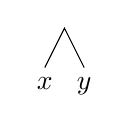
\begin{tikzpicture}[baseline=0cm]
    \node (1) at (-0.25, 0)[below]{\(x\)};
    \node (2) at (+0.25, 0)[below]{\(y\)};

    \draw[-] (-0.25, 0) -- (0, 0.5) -- (+0.25, 0);
  \end{tikzpicture}
  we have that
  \begin{equation*}
    F^00 = \emptyset,
  \end{equation*}
  \begin{equation*}
    F^10 = \emptyset \times \emptyset + 1 = 1 = \{ \bullet \},
  \end{equation*}
  \begin{equation*}
    F^20 = 1 \times 1 + 1 = \left\{ \bullet, 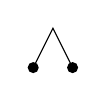
\begin{tikzpicture}[baseline=0cm]
      \draw[-] (-0.25, 0) -- (0, 0.5) -- (+0.25, 0);
      \fill (-0.25, 0) circle (2pt);
      \fill (0.25, 0) circle (2pt);
    \end{tikzpicture}\right\},
  \end{equation*}
    \begin{equation*}
      F^30 = (1 \times 1 + 1) \times (1 \times 1 + 1) + 1 = \left\{ \bullet, 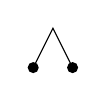
\begin{tikzpicture}[baseline=0cm]
      \draw[-] (-0.25, 0) -- (0, 0.5) -- (+0.25, 0);
      \fill (-0.25, 0) circle (2pt);
      \fill (0.25, 0) circle (2pt);
    \end{tikzpicture},
    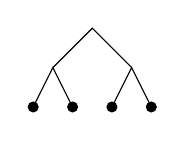
\begin{tikzpicture}[baseline=0cm]
      \fill (-0.75, 0) circle (2pt);
      \fill (-0.25, 0) circle (2pt);
      \fill (0.25, 0) circle (2pt);
      \fill (0.75, 0) circle (2pt);

      \draw (-0.75, 0) -- (-0.5, 0.5) -- (-0.25, 0);
      \draw (0.75, 0) -- (0.5, 0.5) -- (0.25, 0);
      \draw (-0.5, 0.5) -- (0, 1) -- (0.5, 0.5);
    \end{tikzpicture},
    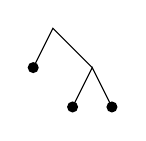
\begin{tikzpicture}[baseline=0cm]
      \fill (0, 0.5) circle (2pt);
      \fill (0.5, 0) circle (2pt);
      \fill (1, 0) circle (2pt);

      \draw (0, 0.5) -- (0.25, 1) -- (0.75, 0.5);
      \draw (0.5, 0) -- (0.75, 0.5) -- (1, 0);
    \end{tikzpicture},
    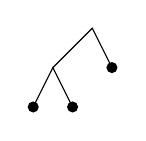
\begin{tikzpicture}[baseline=0cm]
      \fill (0, 0.5) circle (2pt);
      \fill (-0.5, 0) circle (2pt);
      \fill (-1, 0) circle (2pt);

      \draw (0, 0.5) -- (-0.25, 1) -- (-0.75, 0.5);
      \draw (-0.5, 0) -- (-0.75, 0.5) -- (-1, 0);
    \end{tikzpicture}\right\}, \ldots
  \end{equation*}
  so \(F^n0\) is the set of binary trees of height less than \(n\).
  The connecting arrows \(F^n0 \to F^{n+1}0\) are inclusions and so the colimit of the chain, and thus the initial algebra, is the union \(\bigcup_{n<\omega}F^n0\) i.e. the set of all finite binary trees.

  Recall (again from Example \ref{ex:finite_binary_trees}) that the structure \(\iota : \mu F \times \mu F + 1 \to \mu F\) is given by tree-tupling.
  This information too can be obtained by Adámek's Theorem.
  Recall from the proof that, if \((\mu F, c_n: F^n0 \to \mu F)_{i<\omega}\) is the colimit of the initial-algebra \(\omega\)-chain, then \(\iota\) is the unique arrow such that
  \begin{equation}
    \label{eq:cocone_condition}
    c_n = \iota \circ Fc_{n-1} \quad \text{for all \(0 < n < \omega\)}
  \end{equation}
  and, moreover, the \(c_n\)'s are inclusions.
  Now fix \(0 < k < \omega\) and consider a tree
  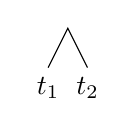
\begin{tikzpicture}[baseline=0cm]
    \node (1) at (-0.25, 0)[below]{\(t_1\)};
    \node (2) at (+0.25, 0)[below]{\(t_2\)};
    \draw[-] (-0.25, 0) -- (0, 0.5) -- (+0.25, 0);
  \end{tikzpicture}
  in \(F^k0\) that we also regard as the pair \((t_1, t_2)\) for \(t_1, t_2 \in F^{k-1}0\).
  We have
  \begin{align*}
    c_k(
    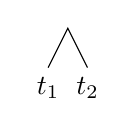
\begin{tikzpicture}[baseline=0cm]
      \node (1) at (-0.25, 0)[below]{\(t_1\)};
      \node (2) at (+0.25, 0)[below]{\(t_2\)};
      \draw[-] (-0.25, 0) -- (0, 0.5) -- (+0.25, 0);
    \end{tikzpicture}
    ) &=
        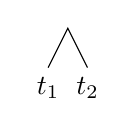
\begin{tikzpicture}[baseline=0cm]
          \node (1) at (-0.25, 0)[below]{\(t_1\)};
          \node (2) at (+0.25, 0)[below]{\(t_2\)};
          \draw[-] (-0.25, 0) -- (0, 0.5) -- (+0.25, 0);
        \end{tikzpicture}
         \in \mu F\\
    \iota \circ Fc_{k-1}((t_1, t_2)) &= \iota(\underbrace{(t_1, t_2)}_{\in \mu F \times \mu F + 1})
  \end{align*}
  so by (\ref{eq:cocone_condition}) \(\iota\) is indeed tree-tupling.
\end{example}

\begin{example}
  For a finite signature \(\Sigma\) the associated polynomial functor \(H_\Sigma\) preserves colimits of \(\omega\)-chains so we can build \(\mu F\), the set of finite \(\Sigma\)-trees, as the colimit of
  \begin{equation*}
    \begin{tikzcd}[sep = large]
      0 \ar[r] & H_\Sigma0 \ar[r] & H_\Sigma^20 \ar[r] & H_\Sigma^30 \ar[r] & \cdots .
    \end{tikzcd}
  \end{equation*}
  Now \(H^n_\Sigma0\) can be regarded as the set of finite \(\Sigma\)-trees of height less than \(n\) while the connecting arrows of the chain are inclusions; thus \(\mu F = \bigcup_{n < \omega}H^n_\Sigma0\) i.e. \(\mu F\) is the set of all finite \(\Sigma\)-trees.
  By an argument similar to that of Example \ref{ex:iota_by_pieces} one can show that the structure \(\iota : H_\Sigma\mu F
  \to \mu F\) is really tree-tupling, as we know from Proposition \ref{prop:finite_sigma_trees}.
\end{example}

\begin{example}
  \label{ex:finite_powerset_adamek}
  The finite power-set functor \(\mathcal{P}_\textsf{f} \colon \Set \to \Set\) preserves colimits of \(\omega\)-chains so it has an initial algebra \(\mu \mathcal{P}_\textsf{f}\) that is the colimit of the following \(\omega\)-chain
  \begin{equation*}
    \begin{tikzcd}[sep = large]
      \emptyset \ar[r] & \{\emptyset\} \ar[r] & \{\emptyset, \{\emptyset\}\} \ar[r] & \{\emptyset, \{\emptyset\}, \{\emptyset, \{\emptyset\}\}\} \ar[r] & \cdots
    \end{tikzcd}
  \end{equation*}
  where the arrows are inclusions.
  We thus obtain that \(\mu F = \bigcup_{n<\omega} \mathcal{P}_\textsf{f}^n0 = V_\omega\); moreover notice that \(\mathcal{P}_\textsf{f}V_\omega\) is precisely \(V_\omega\).
  Now let \((V_\omega, c_n : V_n \to V_\omega)_{i < \omega}\) be the colimit cocone; we know that \(c_n = \iota \circ \mathcal{P}_\textsf{f}c_{n-1}\) for all \(0 < n < \omega\).
  Fix \(0 < n < \omega\) and consider \(\{A_1, \ldots, A_k\} \in V_n\); we have
  \begin{equation*}
    \mathcal{P}_\textsf{f}c_{n-1}(\{A_1, \ldots, A_k\}) = \{c_{n-1}(A_1), \ldots, c_{n-1}(A_k)\} = \{A_1, \ldots, A_k\}
  \end{equation*}
  because \(c_{n - 1}: V_{n-1} \to V_\omega\) is an inclusion.
  Then
  \begin{equation*}
    \iota \circ \mathcal{P}_\textsf{f}c_{n-1}(\{A_1, \ldots, A_k\}) = c_n(\{A_1, \ldots, A_k\}) \Rightarrow \iota(\{A_1, \ldots, A_k\}) = \{A_1, \ldots, A_k\}
  \end{equation*}
  so we obtain \(\iota = \id_{V_\omega}\).
\end{example}

\section{Algebraically Complete Categories}

\begin{definition}
  A category \(\A\) is \textbf{algebraically complete} \marginnote{algebraically complete category} if every endofunctor on it has an initial algebra.
\end{definition}

\begin{remark}
  By the Knaster-Tarski Theorem (see Theorem \ref{teo:knaster_tarski}) every complete lattice is an algebraically complete category.
\end{remark}

The following Theorem shows that, even for categories with very little structure (the existence of products is enough), being algebraically complete is a very strong condition.
The theorem was first proven by Adámek and Koubek in \cite{Adamek-Koubek-1979} (1979); we present a neat proof by Freyd, published in \cite{freyd-1991} (1991).

\begin{theorem}
  Let \(\A\) be an algebraically complete category with products.
  Then \(\A\) is a preorder.
\end{theorem}

\begin{proof}
  Towards a contradiction suppose \(\A\) is not a preorder i.e. there is some hom-set \(\A(A, B)\) that has at least two elements.
  Consider the endofunctor
  \begin{equation*}
    \begin{tikzcd}[sep=large]
      F : \A \ar[r, "{\A(A, -)}"] & \Set \ar[r, "{\Set(-, 2)}"] & \Set^\op \ar[r, "B^{(-)}"] & \A
    \end{tikzcd}
  \end{equation*}
  where \(B^{(-)}: \Set^\op \to \A\) is the functor that takes a set \(M\) to the object
  \begin{equation*}
    B^M = \underbrace{B \times \ldots \times B}_{|M| \text{ times}}.
  \end{equation*}
  We will write \(FD = B^{S(D)}\) for \(S(D) = 2^{\A(A, D)}\).
  Note that \(F\) has no fixed point.
  Indeed assume \(D \cong FD\) then we have
  \begin{align*}
    \A(A, D) & \cong \A(A, FD) && \text{functors preserve isomorphisms}\\
             & \cong \A(A, B^{S(D)}) &&\\
             & \cong \A(A, B)^{S(D)} && \text{hom-functor preserves limits}
  \end{align*}
  but the cardinality of the latter is at least \(2^{|S(D)|} = 2^{2^{|\A(A, D)|}}\) that is impossible by Cantor's Theorem.
  Now Lambeck's Lemma (see Lemma \ref{lemma:lambeck}) gives that \(F\) has no initial algebra thus \(\A\) is not algebraically complete; contradiction.
\end{proof}

\chapter{Initial algebras from transfinite iteration}
\newpage

\section{Colimits of chains}

Through this chapter we regard ordinals \(j \in \Ord\) as linear orders and thus as categories.
A \(j\)-chain in some category \(\A\) is a functor \(C : j \to \A \)\marginnote{\(j\)-chain}; we denote the elements of the chain by \(C_i\), for \(i \in j\), and its arrows by \(c_{i,i'} : C_i \to C_{i'}\) for \(i \leq i' < j\).
We say that \(\A\) has colimits of chains if for all \(j \in \Ord\) every \(j\)-chain has a colimit; this includes the existence of an initial object (as the colimit of the empty chain) but does not include colimits of \(\Ord\)-chains.

\begin{lemma}
  \label{lemma:final_functors}
  Let \(j\) be an ordinal and \(C : j \to \A\) a \(j\)-chain into a category \(\A\) with colimits of chains.
  Now let \(j' \subseteq j\) be cofinal in \(j\) i.e. such that for every \(i \in j\) there is some \(i' \in j'\) such that \(i \leq i'\) and denote by \(C'\) the restriction of \(C\) to \(j'\).
  Then \(C\) and \(C'\) have the same colimit.
\end{lemma}

\begin{proof}
  Notice that there is a canonical bijection between cocones on \(C\) and cocones on \(C'\).
  Given a cocone \((A, \alpha_i : C_i \to A)_{i \in j}\) on \(C\) throwing away all the indexes not in \(j'\) yields \((A, \alpha_i : C_i \to A)_{i \in j'}\): a cocone on \(C'\).
  Conversely given \((A, \alpha_i : C_i \to A)_{i \in j'}\) we need to define \(\alpha_i : C_i \to A\) for all \(i \in j \setminus j'\); but there's only one way to do so.
  Indeed by cofinality let \(i' \in j'\) be such that \(i \leq i'\); then by the cocone condition we must set \(\alpha_i = \alpha_{i'} \circ c_{i,i'}\).
  This is independent of the choice of \(i'\) since if \(i \leq i' < i''\) with \(i', i'' \in j'\) then we have
  \begin{equation*}
    \alpha_i = \alpha_{i'} \circ c_{i, i'} = \alpha_{i''} \circ c_{i', i''} \circ c_{i, i'} = \alpha_{i''} \circ c_{i, i''}.
  \end{equation*}
  Thus \((A, \alpha_{i}:C_i \to A)_{i \in j'}\) can be extended to the whole chain in only one way.

  Let \((L, \sigma_i : C_i \to L)_{i \in j}\) be the colimit of \(C\); then \((L, \sigma_i : C_i \to L)_{i \in j'}\) is the colimit of \(C'\).
  Indeed let \((A, \alpha_i : C_i \to A)_{i \in j'}\) be a cocone on \(C'\) that we extend to a cocone on \(C\) as explained above.
  Now, since \(L\) is the colimit, let \(m \colon L \to A\) be the unique factorization arrow such that
  \begin{equation*}
    m \circ \sigma_i = \alpha_i \quad \text{for all \(i \in j\)}.
  \end{equation*}
  Particularly for all \(i \in j'\) so \(m\) is a factorization of \((A, \alpha_i : C_i \to A)_{i \in j'}\) through \((L, \sigma_i : C_i \to L)_{i \in j'}\).
  To prove it is unique let \(n \colon L \to A\) be such that \(n \circ \sigma_i = \alpha_i\) for all \(i \in j'\); we will show that \(n\) actually works for all \(i \in j\) and thus must be \(m\) by uniqueness.
  Let \(i \in j \setminus j'\) and \(i' \in j'\) such that \(i \leq i'\) by cofinality, then we have
  \begin{equation*}
    n \circ \sigma_i = n \circ \sigma_{i'} \circ c_{i, i'} = \alpha_{i'} \circ c_{i,i'} = \alpha_i.
  \end{equation*}
  For the converse let \((L, \sigma_i : C_i \to L)_{i \in j'}\) be the colimit of \(C'\).
  One can prove that its unique extension \((L, \sigma_i : C_i \to L)_{i \in j}\) is the colimit of \(C\) by an argument similar to the one above.
  Finally we have that \(C\) and \(C'\) have the same colimit (modulo restriction/extension) and, moreover, the factorization arrows are the same.
\end{proof}

Thanks to this lemma we can safely calculate colimits of chains, or apply Proposition \ref{prop:arrows_from_colimit}, on convenient cofinal subchains.
This will allow us to ``skip'' limit ordinals because given \(j\) limit the subset \(\{i \in j : \text{\(i\) successor}\}\) is cofinal in \(j\).

\section{Transfinite iteration}

The main result of this section is again a generalization to the categorical setting of an order-theoretic result; this time from Zermelo (see \cite{zermelo}).
Let \(P\) be a chain-complete poset (particularly it has a bottom element \(\bot\)) and \(f : P \to P\) an order-preserving map.
We can define an \(\Ord\)-indexed sequence by transfinite recursion as follows
\begin{align*}
  f^0(\bot) = \bot && \text{base case;}\\
  f^{j+1}(\bot) = f(f^j(\bot)) && \text{for all ordinals \(j\);} \\
  f^j(\bot) = \bigvee_{i < j}f^i(\bot) && \text{for limit ordinals \(j\).}
\end{align*}
This sequence is clearly a chain.

\begin{theorem}[Zermelo]
  \label{teo:Zermelo}
  Let \(P\) be a chain-complete poset.
  Then every order-preserving \(f : P \to P\) has a lest fixed point \(\mu f\) and \(\mu f = f^j(\bot)\) for some \(j \in \Ord\).
\end{theorem}

\begin{proof}
  By Hartog's Lemma (see \cite[Theorem 8.18]{goldrei} for a proof) there is an ordinal \(i\) such that there is no injection \(i \rightarrowtail P\).
  Particularly the function \(i \to P\) defined by \(j \mapsto f^j(\bot)\) is not injective thus there are \(j < k < i\) such that \(f^j(\bot) = f^k(\bot)\) and we have \(f^j(\bot) \leq f^{j+1}(\bot) \leq f^k(\bot)\) because \((f^j(\bot))_{j\in\Ord}\) is a chain.
  So \(f(f^j(\bot)) = f^{j+1}(\bot) = f^j(\bot)\) hence \(f^j(\bot)\) is a fixed point.

  Now let \(x = f(x)\) be another fixed point.
  By transfinite induction we can prove \(x \geq f^i(\bot)\) for all \(i \in \Ord\) (similarly to what we did in Theorem \ref{teo:kleene})\footnote{\color{teal} Ora abbiamo richiamato nel paragrafo precedente che \(\bot\) è il bottom e che \(P\) ne è dotato perché chain-complete. È necessario ribadirlo qui?} thus when \(i = j\) we obtain \(x \geq f^j(\bot)\).
  This proves that \(f^j(\bot)\) is indeed the least fixed point of \(f\).
\end{proof}

In order to generalize this theorem and its proof we begin by defining a trasfinite version of the initial-algebra \(\omega\)-chain.
This will be a functor \(W : \Ord \to \A\) into a category \(\A\) with colimits of chains.
It is defined by transfinite recursion as follows.
\begin{align*}
  W_0 = 0 && \text{base case};\\
  W_{j+1} = FW_j && \text{for all ordinals \(j\)};\\
  W_j = \colim_{i < j}W_i && \text{for all limit ordinals \(j\)}.
\end{align*}
As for arrows \(w_{0,1}\) is the unique arrow \(0 \to W_1 = F0\) and \(w_{i + 1, j+1} = Fw_{i,j}\) for all \(i, j \in \Ord\).
When \(j\) is limit we have \(W_j = \colim_{i < j}W_i\) so we let \(\{w_{i,j}\}_{i < j}\) be the arrows forming the colimit cocone.
We are only missing \(w_{j, j+1}\) for \(j\) limit.
Such arrows are obtained using the universal property of \(W_j\).
First notice that we can leave out the initial object \(0\) and all the limit ordinals without changing the colimit i.e.
\begin{equation*}
  W_j = \colim_{i < j}W_i = \colim_{\text{\(i < j\) successor}}W_i
\end{equation*}
by Lemma \ref{lemma:final_functors}.
Now \((Fw_{i,j} : FW_i = W_{i+1} \to FW_{j} = W_{j+1})_{i < j}\) is a cocone on this reduced diagram.
Thus we obtain a unique factorization arrow \(W_j \to W_{j+1}\) that we clare to be our \(w_{j, j+1}\) so the definition of our transfinite chain can continue.
Notice also that, being the factorization arrow, \(w_{j, j_+1}\) is such that
\begin{equation}
  \label{eq:omega-to-omega-plus-one}
  w_{j, j+1} \circ w_{i+1, j} = Fw_{i, j} \quad \text{for all \(i < j\)}.
\end{equation}

We now generalize Remark \ref{rem:induced_cocone} to the transfinite case.

\begin{remark}
  \label{rem:induce-transfinite-cocone}
  Let \((A, \alpha)\) be an \(F\)-algebra; then it induces a cocone \((\alpha_i : W_i \to A)_{i \in \Ord}\) on \(W\) as follows.
  \begin{align*}
    \alpha_0 &=\ ! && \text{base case};\\
    \alpha_{i+1} &= \alpha \circ F\alpha_i && \text{for all ordinals i};
  \end{align*}
  for limit ordinals \(j\) we define \(\alpha_{j} : W_j \to A\) to be the unique factorization arrow such that \(\alpha_j \circ w_{i,j} = \alpha_i\) for all \(i < j\).
  In order for this construction to work we need to prove that, at stage \(j\), \((\alpha_i : W_i \to A)_{i < j}\) is a cocone i.e. that
  \begin{equation}
    \label{eq:cocone-condition}
    \alpha_i \circ w_{k, i} = \alpha_{k}
  \end{equation}
  for all \(k < i < j\).
  Assuming that all \(\alpha_i\)'s for \(i < j\) have been constructed we have that:
  \begin{itemize}
  \item[1.] for \(w_{0,1}\) condition (\ref{eq:cocone-condition}) is trivial;
  \item[2.] for \(w_{k, i}\) with \(i\) limit it is trivial by construction of \(\alpha_{i}\);
  \item[3.] for \(w_{i, i+1}\) with \(i\) limit we can prove (\ref{eq:cocone-condition}) holds by showing
    \[\alpha_{i+1} \circ w_{i, i+1} \circ w_{k, i} = \alpha_i \circ w_{k, i} =  \alpha_{k}\]
    for all \(k < i\) and conclude by uniqueness of \(\alpha_i\).
    It is enough to prove the relation for all \(k < i\) successors by Lemma \ref{lemma:final_functors} and indeed we have
    \begin{align*}
      \alpha_{i+1} \circ w_{i, i+1} \circ w_{k, i} &= \alpha \circ F\alpha_i \circ w_{i, i+1} \circ w_{k, i} && \text{definition of \(\alpha_{i+1}\)}\\
                                      &= \alpha \circ F\alpha_i \circ Fw_{k-1, i} && \text{(\ref{eq:omega-to-omega-plus-one})} \\
                                      &= \alpha \circ F(\alpha_i \circ w_{k-1, i}) && \text{functoriality of \(F\)}\\
                                      &= \alpha \circ F\alpha_{k-1} && \text{definition of \(\alpha_{i}\)}\\
                                      &= \alpha_k && \text{definition of \(\alpha_k\)}.
    \end{align*}
  \item[4.] for \(w_{i,i+1}\) with \(i\) non-limit we proceed inductively like in Remark \ref{rem:induced_cocone}; the base case is provided by item 1 if \(i\) is a natural number and by item 3 otherwise.
  \end{itemize}
  Finally we conclude that \((\alpha_i : W_i \to A)_{i \in \Ord}\) is well defined and a cocone on \(W\) since, as we just proved, for every \(j\) limit \((\alpha_i : W_i \to A)_{i < j}\) is a cocone.
\end{remark}

\begin{definition}
  We say that the inital-algebra chain \textbf{converges}
  \marginnote{convergence of the initial-algebra chain}
  in \(\lambda\) steps if \(w_{\lambda, \lambda+1}\) is an isomorphism and that it converges in \textbf{exactly} \(\lambda\) steps when \(\lambda\) is the least such ordinal.
\end{definition}

We are now ready to state and prove the transfinite version of Adámek's Theorem.

\begin{theorem}
  \label{teo:adamek_transfinite}
  Let \(\A\) be a category with colimits of chains and \(F\) an endofunctor.
  If the initial-algebra chain of \(F\) converges in \(j\) steps then \(W_j\) is the initial algebra \(\mu F\) with structure given by
  \begin{equation*}
    (w_{j,j+1})^{-1} : W_{j+1} = FW_j \to W_j.
  \end{equation*}
\end{theorem}

\begin{proof}
  We only need to prove that \(W_j\) with the algebra structure given above is initial.
  To this end let \((A, \alpha)\) be an \(F\)-algebra and let \(h\) be the arrow \(\alpha_j : W_j \to A\) of the cocone induced by \((A, \alpha)\) in the sense of Remark \ref{rem:induce-transfinite-cocone}.
  We shall prove that \(h\) is the unique \(F\)-algebra homomorphism from \(W_j\) to \(A\).
  \begin{equation*}
    \begin{tikzcd}[sep=huge]
      W_{j+1} = FW_j \ar[r, "(w_{j,j+1})^{-1}"] \ar[d, "Fh = F\alpha_j"'] \ar[dr, "\alpha_{j+1}"] & W_j \ar[d, "h = \alpha_j"]\\
      FA \ar[r, "\alpha"] & A
    \end{tikzcd}
  \end{equation*}
  In the above diagram the lower left triangle commute by construction of \(\alpha_{j+1}\) and the upper right one because the \(\alpha_i\)'s form a cocone.
  Thus the outer square commutes i.e. \(h\) is an homomorphism.

  To prove that \(h\) is unique assume that \(k : W_j \to A\) is another homomorphism.
  We will show by transfinite induction that \(h \circ w_{i, j} = k \circ w_{i, j}\) for all \(i \leq j\) and then conclude by choosing \(i = j\).
  Notice that \(h \circ w_{i, j} = \alpha_j \circ w_{i, j} = \alpha_i\) so we are really interested in proving
  \begin{equation}
    \label{eq:a}
    \alpha_i = k \circ w_{i, j}
  \end{equation}
  for all \(i \leq j\).
  If \(i = 0\) then (\ref{eq:a}) is obvious because both sides are arrows out of the initial object.
  If we have \(\alpha_i = k \circ w_{i, j}\) then
  \begin{align*}
    \alpha_{i+1} &= \alpha \circ F\alpha_i && \text{definition of \(\alpha_i\)}\\
            &= \alpha \circ F(k \circ w_{i, j}) && \text{inductive hypothesis}\\
            &= \alpha \circ Fk \circ w_{i+1, j+1} && \text{fuctoriality of \(F\)}\\
            &= k \circ (w_{j,j+1})^{-1} \circ w_{i+1, j+1} && \text{\(k\) is an homomorphism}\\
            &= k \circ w_{i+1, j}.
  \end{align*}
  Finally if \(i\) is limit we know \(\alpha_i\) is the unique arrow such that \(\alpha_i \circ w_{s,i} = \alpha_s\) for all \(s < i\); so if we show that \(k \circ w_{i, j}\) does the same then we have (\ref{eq:a}).
  Indeed for \(s < i\) we have
  \begin{align*}
    k \circ w_{i, j} \circ w_{s, i} &= k \circ w_{s, j} && \\
                            &= h \circ w_{s, j} && \text{inductive hypothesis since \(s < i\)}\\
                            &= \alpha_j \circ w_{s, j} && \\
                            &= \alpha_s && \text{the \(\alpha_i\)'s are a cocone}.
  \end{align*}
  This concludes the proof.
\end{proof}

\begin{corollary}
  \label{coroll:adamek}
  Let \(\A\) be a category with colimits of chains and \(F\) an endofuctor.
  If \(F\) preserves colimits of \(\lambda\)-chains for some limit ordinal \(\lambda\) then the initial algebra chain of \(F\) converges in \(\lambda\) steps.
  Therefore we have \(\mu F = W_\lambda\).
\end{corollary}

\begin{proof}
  Since \(W_\lambda = \colim_{i < \lambda} W_i\) and \(F\) preservers colimits of \(\lambda\)-chains we have that \(FW_\lambda = \colim_{i < \lambda} FW_i\) with colimit cocone \((Fw_{i, \lambda} = w_{i+1, \lambda + 1}: W_{i+1} \to W_{\lambda+1} = FW_\lambda)_{i < \lambda}\).
  We thus obtain a unique morphism \(\iota : W_{\lambda+1} = FW_\lambda \to W_\lambda\) such that \(\iota \circ Fw_{i, \lambda} = w_{i+1, \lambda}\) for all \(i < \lambda\) (similarly to the proof of Theorem \ref{teo:adamek}).
  Combining this universal property with that of \(w_{\lambda, \lambda + 1}\) (see \ref{eq:omega-to-omega-plus-one}) we obtain the following two identities for all \(i < \lambda\).
  \begin{align*}
    \iota \circ Fw_{i, \lambda} = w_{i+1, \lambda} & \implies \iota \circ w_{\lambda, \lambda + 1} \circ w_{i+1, \lambda} = \id_{W_\lambda} \circ w_{i+1, \lambda} \\
    w_{\lambda, \lambda+1} \circ w_{i+1, \lambda} = Fw_{i, \lambda} &\implies w_{\lambda, \lambda+1} \circ \iota \circ Fw_{i, \lambda} = \id_{W_{\lambda+1}} \circ Fw_{i, \lambda}
  \end{align*}
  And, by Proposition \ref{prop:arrows_from_colimit}, \(\iota \circ w_{\lambda, \lambda+1} = \id_{W_\lambda}\) and \(w_{\lambda, \lambda+1} \circ \iota = \id_{W_{\lambda+1}}\) so the inital-algebra chain converges in \(\lambda\) steps.
  We conclude by Theorem \ref{teo:adamek_transfinite}.
\end{proof}

Clearly for \(\lambda = \omega\) we obtain Adámek's Theorem.
We now give an example of a functor that has initial-algebra convergent in more than \(\omega\) steps; showing that Theorem \ref{teo:adamek_transfinite} is more powerful than Adámek's Theorem.

\begin{example}
  Recall that trees are simple graphs such that every two distinct vertexes are connected by a unique path; we generally mark one vertex as the \textbf{root} of the tree and draw them with the root on top as we have been doing so far.
  Trees with no infinite paths are called \textbf{well-founded}.\marginnote{well-founded tree}
  When a tree \(t\) is well-founded we define its \textbf{height}\marginnote{height of a tree} by
  \begin{equation*}
    h(t) = \sup \{h(t') + 1 : \quad t' \text{ maximal proper subtree of \(t\)}\}.
  \end{equation*}
  Thus finite trees (that are always well-founded) have height equal to the maximum length of a root-to-leaf path.
  For other trees the height is an infinite ordinal: \(T_1\) below is constructed by linking to the root a copy of every path of finite length; thus the height of \(T_1\) is \(\omega\).
  On the other hand \(T_2\) has \(T_1\) as the only maximal proper subtree so its height is \(\omega + 1\).
  \setlength{\tabcolsep}{20pt}
  \begin{center}
    \begin{tabular}{ c c }
      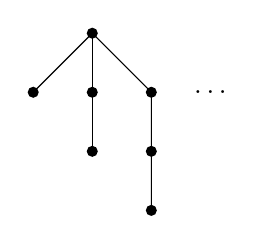
\begin{tikzpicture}
        \fill (0, 0) circle (2pt);
        \fill (0.75, 0) circle (2pt);
        \fill (0.75, -0.75) circle (2pt);
        \fill (1.5, 0) circle (2pt);
        \fill (1.5, -0.75) circle (2pt);
        \fill (1.5, -1.5) circle (2pt);
        \fill (0.75 ,0.75) circle (2pt);
        \node (dots) at (2.25, 0){\(\ldots\)};

        \draw (0.75 ,0.75) -- (0, 0);
        \draw (0.75 ,0.75) -- (0.75, -0.75);
        \draw (0.75 ,0.75) -- (1.5, 0) -- (1.5, -1.5);
      \end{tikzpicture}
        &       \begin{tikzpicture}
        \fill (0, 0) circle (2pt);
        \fill (0.75, 0) circle (2pt);
        \fill (0.75, -0.75) circle (2pt);
        \fill (1.5, 0) circle (2pt);
        \fill (1.5, -0.75) circle (2pt);
        \fill (1.5, -1.5) circle (2pt);
        \fill (0.75 ,0.75) circle (2pt);
        \fill (0.75 ,1.5) circle (2pt);
        \node (dots) at (2.25, 0){\(\ldots\)};

        \draw (0.75 ,1.5) -- (0.75, 0.75);
        \draw (0.75 ,0.75) -- (0, 0);
        \draw (0.75 ,0.75) -- (0.75, -0.75);
        \draw (0.75 ,0.75) -- (1.5, 0) -- (1.5, -1.5);
      \end{tikzpicture} \\
      \(T_1\) & \(T_2\)
    \end{tabular}
  \end{center}
  We have seen in Example \ref{ex:iota_by_pieces} that \(FX = X \times X + 1\) on \(\Set\) satisfies the hypothesis of Adámek's Theorem \ref{teo:adamek} thus from Corollary \ref{coroll:adamek} its initial-algebra chain converges in \(\omega\) steps to the algebra of finite binary trees.
  Now consider the functor \(GX = X^\omega + 1\) on \(\Set\).
  Its initial-algebra chain is given by
  \begin{equation*}
    W_i = \{\text{all countably branching trees \(t\) such that \(h(t) < i\)}\}
  \end{equation*}
  and the connecting arrows are inclusions.
  Indeed \(W_0 = \emptyset\), \(W_1 = \{t_0\}\) where \(t_0\) is the root-only tree (the unique tree of height 0), \(W_2 = W_1^\omega + 1\) contains the root-only tree, of height 0, and the unique countably branching tree
  \begin{equation*}
    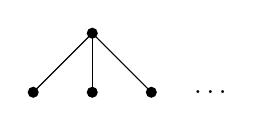
\begin{tikzpicture}
      \fill (0, 0) circle (2pt);
      \fill (0.75, 0) circle (2pt);
      \fill (1.5, 0) circle (2pt);
      \fill (0.75 ,0.75) circle (2pt);
      \node (dots) at (2.25, 0){\(\ldots\)};
      
      \draw (0.75 ,0.75) -- (0, 0);
      \draw (0.75 ,0.75) -- (0.75, 0);
      \draw (0.75 ,0.75) -- (1.5, 0);
    \end{tikzpicture}
  \end{equation*}
  of height 1.
  Generally \(W_{i + 1} = (W_i)^\omega + 1\) gives us that the elements of \(W_{i+1}\) are the root-only tree and all trees
  \begin{equation*}
    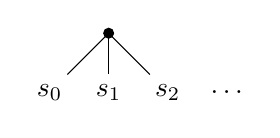
\begin{tikzpicture}
      \fill (0.75, 0.75) circle (2pt);
      \node (1) at (0, 0){\(s_0\)};
      \node (2) at (0.75, 0){\(s_1\)};
      \node (3) at (1.5 ,0){\(s_2\)};
      \node (dots) at (2.25, 0){\(\ldots\)};
      
      \draw (0.75 ,0.75) -- (1);
      \draw (0.75 ,0.75) -- (2);
      \draw (0.75 ,0.75) -- (3);
    \end{tikzpicture}
  \end{equation*}
  where \(s_n \in W_i\) for every \(n < \omega\).
  Since the connecting maps \(w_{i, i+1}\) are inclusions at limit steps we take unions so, for example, \(W_\omega\) is the set of all countably branching trees of height less than \(\omega\) i.e. all countably branching trees of finite height.
  However, as opposed to what happens for \(F\), the chain does not stop at \(\omega\) because one can take a sequence \(t_0, t_1, t_2, \ldots\) of trees with heights cofinal in \(\omega\); then the tree
  \begin{equation}
    \label{eq:tree}
    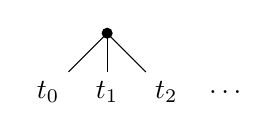
\begin{tikzpicture}
      \fill (0.75, 0.75) circle (2pt);
      \node (1) at (0, 0){\(t_0\)};
      \node (2) at (0.75, 0){\(t_1\)};
      \node (3) at (1.5 ,0){\(t_2\)};
      \node (dots) at (2.25, 0){\(\ldots\)};
      
      \draw (0.75 ,0.75) -- (1);
      \draw (0.75 ,0.75) -- (2);
      \draw (0.75 ,0.75) -- (3);
    \end{tikzpicture}
  \end{equation}
  has height \(\omega\) i.e. it is an element of \(W_{\omega+1} \setminus W_\omega\).
  Indeed for every countable ordinal \(i < \omega_1\), by the same argument, one has that \(W_{i} \subset W_{i+1}\).
  The chain then converges at the first uncountable ordinal \(\omega_1\) because, given a sequence of trees \(t_0, t_1, t_2, \ldots\) such that \(t_n \in W_{i_n}\) for \(i_n < \omega_1\) then the tree (\ref{eq:tree}) has height \(\sup\{i_0, i_1, i_2, \ldots\}\) that is a countable ordinal, and thus \(t \in W_{\omega_1}\).
  So the initial-algebra \(\mu G\) is the set of all well-founded countable branching trees.
\end{example}

\section{Smooth monomorphisms and a converse to Lambeck's Lemma}

From Theorem \ref{teo:adamek_transfinite} we know that convergence of the initial-algebra chain implies existence of the initial algebra; but what about the converse?
Are all initial algebras obtainable by iteration?
The following example shows that this is not the case.
\begin{example}
  A graph \(G\) is a pair \((V_G, E_G)\) where \(V_G\) is a set of vertexes and \(E_G\) a symmetric binary relation on \(V_G\).
  When \(x E_G y\) we say that \(x\) and \(y\) are adjacent.
  A graph morphism is a function \(f : G \to G'\) such that \(x E_G y\) implies \(f(x) E_{G'} f(y)\) for every \(x, y \in V_G\).
  Graphs and graph morphisms form the category \(\textsf{Gra}\).

  We say that a graph \(G\) has a loop if there is some vertex \(x\) such that \(x E_G x\) and that it is loop-free otherwise.
  For a cardinal \(\kappa\) we denote by \(K_\kappa\) the loop-free graph on \(\kappa\) vertexes such that any two distinct vertexes are always adjacent; these graphs are called complete graphs.
  Given a loop-free graph \(G\) we define its chromatic number \(\chi(G)\) to be the smallest cardinal such that there is a morphism from \(G\) to \(K_{\chi(G)}\); notice that \(\chi(K_\kappa) = \kappa\).
  Finally we can consider the following endofunctor on \(\textsf{Gra}\):
  \begin{equation*}
    FG = \begin{cases}
      1 & \text{if \(G\) has loops}\\
      K_{\kappa^+} & \text{if \(G\) is loop-free}
    \end{cases}
  \end{equation*}
  where \(1\) is the loop on a single vertex and \(\kappa^+\) is the smallest cardinal bigger than \(\kappa = \chi(G) + \aleph_1\).
  As for arrows if we have \(f: G \to G'\) and \(G, G'\) are loop-free then \(Ff\) is the inclusion between complete graphs, otherwise if \(G\) has loops so must \(G'\) and \(Ff\) is \(\text{id}_1\), finally if \(G\) is loop-free and \(G'\) has a loop then \(Ff\) is the constant function to 1.

  If \(G\) is loop-free then there are no arrows from \(FG\) to \(G\) because the existence of such an arrow implies \(\chi(FG) \leq \chi(G)\) but we have \(\chi(FG) > \chi(G)\) by construction of \(F\).
  Then every \(F\)-algebra is of the form \(1 \to G\) with \(G\) a graph that has a loop.
  This means that \(F\)-algebras are graphs \(G\) with a marked loop and it is clear that \(\id_1 : F1 = 1 \to 1\) is the initial algebra.
  However the initial-algebra chain of \(F\) never converges because its elements have increasing cardinalities.
\end{example}

However, in the case of \(\Set\), we have the following result that, together with Lambeck's Lemma, immediately implies that every initial algebra over \(\Set\) is obtained by iteration.

\begin{theorem}
  \label{teo:set_lambeck_converse}
  Let \(F\) be an endofunctor over \(\Set\) such that there is some set \(A\) and an injective function \(\alpha : FA \rightarrowtail A\); then the initial-algebra chain of \(F\) converges.
\end{theorem}

\begin{proof}
  The implication is trivial if \(F\emptyset = \emptyset\) (Remark \ref{rem:trivial_initial_algebra}) so we only need to prove the theorem under the assumption that \(F\emptyset \neq \emptyset\).

  Our \(\alpha : FA \rightarrowtail A\) is an \(F\)-algebra so it induces a canonical cocone \((\alpha_i:W_i \to A)_{i \in \Ord}\) over the initial-algebra chain \((W_i)_{i \in \Ord}\) as of Remark \ref{rem:induce-transfinite-cocone}; we will prove that \(\alpha_\omega\) is injective.
  
  Since \(F\emptyset \neq \emptyset\) then, upon the action of the functor, we obtain a function \(F\emptyset \to FA\) with non-empty domain from the unique \(\emptyset \to A\) so \(FA \neq \emptyset\) and, as we have \(\alpha\), by the same argument we get that \(A \neq \emptyset\).
  Now \(\alpha\) is injective so it splits i.e. there exists \(\alpha': A \to FA\) such that \(\alpha' \circ \alpha = \id_{FA}\) and, since \(F\emptyset \neq \emptyset\), let \(u_0\) be any function of type \(A \to F\emptyset\).
  Then we define
  \begin{equation*}
    u_{n+1} = Fu_n \circ \alpha' \quad \text{for \(0 < n < \omega\)}
  \end{equation*}
  and obtain the following situation.
  \begin{equation*}
    \begin{tikzcd}[sep=huge]
      & & A \ar[dl, bend right=10, "u_0"'] \ar[d, shift right=1, "u_1"'] \ar[dr, bend right=10, "u_2"'] & &\\
      \emptyset \ar[urr, bend left=10, "\alpha_0"] \ar[r, "w_{0,1}"'] & F\emptyset \ar[r, "w_{1,2}"'] \ar[ru, bend right=10, "\alpha_1"'] & F^2\emptyset \ar[r, "w_{2, 3}"'] \ar[u, shift right=1, "\alpha_2"'] & F^3\emptyset \ar[r, "w_{3, 4}"'] \ar[lu, bend right=10, "\alpha_3"'] & \cdots
    \end{tikzcd}
  \end{equation*}
  
  We have that \(w_{n, n+1} = u_n \circ \alpha_n\) holds for \(n < \omega\) by induction.
  The base case is obtained by noticing that \(u_0 \circ \alpha_0\) and \(w_{0,1}\) are both arrows of type \(\emptyset \to F\emptyset\) and \(\emptyset\) is the initial object.
  The inductive step follows from the following calculation using the definitions of \(\alpha'\), \(u_{n+1}\), \(\alpha_{n+1}\) and the inductive hypothesis:
  \begin{equation*}
    w_{n+1, n+2} = Fw_{n, n+1} = Fu_n \circ F\alpha_n = (Fu_n \circ \alpha') \circ (\alpha \circ F\alpha_n) = u_{n+1} \circ \alpha_{n+1}.
  \end{equation*}
  Finally let \(x, y \in W_\omega\) such that \(\alpha_\omega(x) = \alpha_\omega(y)\).
  Since \(W_\omega = \colim_{n < \omega}F^n\emptyset\) there is some \(k < \omega\) and \(x', y' \in F^k\emptyset\) such that \(w_{k, \omega}(x') = x\) and \(w_{k, \omega}(y') = y\).
  Then, as \((\alpha_i: W_i \to A)_{i \in \Ord}\) is a cocone, \(\alpha_k = \alpha_\omega \circ w_{k, \omega}\) so \(\alpha_k(x') = \alpha_k(y')\) and we have
  \begin{equation*}
    w_{k+1, \omega} \circ u_k \circ \alpha_k = w_{k+1, \omega} \circ w_{k, k+1} = w_{k, \omega}
  \end{equation*}
  that implies
  \begin{equation*}
    x = w_{k, \omega}(x') = (w_{k+1, \omega} \circ u_k \circ \alpha_k)(x') = (w_{k+1, \omega} \circ u_k \circ \alpha_k)(y') = w_{k, \omega}(y') = y
  \end{equation*}
  and this completes the proof that \(\alpha_\omega\) is injective.
  Now we can prove that the initial-algebra chain converges.

  Since \(\alpha_\omega\) is injective and has non-empty domain there is a function  \(\beta : A \to W_\omega\) such that \(\beta \circ \alpha_\omega  = \id_A\).
  Because of this \(F\alpha_\omega\) is also injective (functors preserve identities and composition)\footnote{\color{teal} Qui usiamo che da \( F\beta \circ F\alpha_\omega = \id_{FA}\) segue che \(F\alpha_\omega\) deve essere iniettiva perché \(\id_{FA}\) lo è. Va detto esplicitamente o basta quanto c'è tra parentesi (con l'uguaglianza prima corretta)?} and so must be \(\alpha_{\omega + 1} = \alpha \circ F\alpha_\omega\).
  If we define \(v = \beta \circ \alpha_{\omega + 1}\) we obtain
  \begin{equation*}
    \alpha_\omega \circ v = \alpha_\omega \circ \beta \circ \alpha_{\omega + 1} = \alpha_{\omega + 1}
  \end{equation*}
  from which
  \begin{equation*}
     \alpha_\omega \circ v \circ w_{\omega, \omega + 1} = \alpha_{\omega + 1} \circ w_{\omega, \omega + 1} = \alpha_\omega \implies v \circ w_{\omega, \omega + 1} = \id_{W_\omega};
  \end{equation*}
  \begin{equation*}
    \alpha_{\omega + 1} \circ w_{\omega, \omega + 1} \circ v = \alpha_{\omega} \circ v = \alpha_{\omega + 1} \implies  w_{\omega, \omega + 1} \circ v = \id_{W_{\omega + 1}}.
  \end{equation*}
  So \(w_{\omega, \omega + 1}\) is an isomorphism and the initial-algebra chain converges.
\end{proof}

Now we'd like to generalize Theorem \ref{teo:set_lambeck_converse}.
Notice that \(\alpha, \alpha_\omega\) and \(\alpha_{\omega + 1}\) being injective (mono) plays a crucial role in the argument above; this suggests that we should look into monomorphisms and, particularly, subobjects.

\begin{definition}
  Fixed an object \(A\) in a category \(\A\) a \textbf{subobject} of \(A\) is represented by a monomorphism \(m: B \rightarrowtail A\) \marginnote{subobject}.
  If we have two monomorphisms \(m_B : B \rightarrowtail A, m_C : C \rightarrowtail A\) we write \(m_B \leq m_C\) if there is some \(k : B \to C\) such that \(m_B = m_C \circ k\) (notice that this \(k\) too is mono).
  When we have \(m_B \leq m_C \leq m_B\) the \(k\) above is an isomorphism and we say \(m_B\) and \(m_C\) represent the same subobject.
  Thus we can consider the collection of equivalence classes of subobjects of \(A\) that is partially ordered by \(\leq\).
  If \(\A\) is such that every object \(A \in \A\) has only a set of subobjects then \(\A\) is called \textbf{well-powered} \marginnote{well-powered category}.
\end{definition}
We can restrict ourselves to a class \(\mathcal{M}\) of monomorphisms and speak of \(\mathcal{M}\)-subobjects i.e. subobjects represented by mono in \(\mathcal{M}\).
When a given object \(A\) has only a set of \(\mathcal{M}\)-subobjects we write \(\Sub_\mathcal{M}(A, \leq)\) \marginnote{\(\Sub_\mathcal{M}(A, \leq)\)} for the poset of \(\mathcal{M}\)-subobjects of \(A\); if \(\mathcal{M}\) is the class of all monomorphisms we also write simply \(\Sub(A, \leq)\).
Notice that we do not require the monomorphisms that witness \(\leq\) to be in \(\mathcal{M}\).

From here onwards let \(\mathcal{M}\) denote \marginnote{\(\mathcal{M}\)} a class of monomorphisms (of some generic category \(\A\) or otherwise clear from the context) containing all isomorphisms and closed under composition.

\begin{definition}
  \label{def:smooth-subobjects}
  We say that an object \(A\) has \textbf{smooth} \(\mathcal{M}\)\textbf{-subobjects} if \(\Sub_\mathcal{M}(A, \leq)\) \marginnote{smooth\\ \(\mathcal{M}\)-subobjects} is a chain-complete poset (particularly it is a set) where joins of chains are given by colimits of the corresponding chain of subobjects.
  We say that the class \(\mathcal{M}\) itself is \textbf{smooth} \marginnote{smooth class of monomorphisms} if every object has smooth \(\mathcal{M}\)-subobjects.
  When the class of all monomorphisms of a given category is smooth we say that the category has \textbf{smooth monomorphisms}.
\end{definition}

\begin{remark}
  \label{rem:classes_and_initial}
  To be more precise consider an ordinal \(\lambda\) and a chain of \(\mathcal{M}\)-subobjects \((m_i : A_i \rightarrowtail A)_{i < \lambda}\) i.e. we have arrows \(a_{i,j} : A_i \to A_j\) (that need not be in \(\mathcal{M}\)) that withness \(m_i \leq m_j\) for \(i \leq j < \lambda\).
  By definition if \(A\) has smooth \(\mathcal{M}\)-subobjects then there is an \(\mathcal{M}\)-subobject \(m : C \rightarrowtail A\) that is the join of our chain in \(\Sub_\mathcal{M}(A, \leq)\).
  Particularly we have that \(m_i \leq m\) for all \(i < \lambda\) so there are morphisms \(c_i : A_i \to C\) such that \(m \circ c_i = m_i\) for all \(i < \lambda\).
  These morphisms form a cocone over our chain: given \(a_{i, j}\) for \(i < j\) we have
  \begin{equation*}
    m \circ c_j \circ a_{i, j} = m_j \circ a_{i, j} = m_i = m \circ c_i
  \end{equation*}
  and so \(c_j \circ a_{i, j} = c_i\) because \(m\) is mono.
  In order to have smooth \(\mathcal{M}\)-subobjects this cocone must be a colimit in \(\A\).

  This gives us another way of interpreting Definition \ref{def:smooth-subobjects}.
  If we consider \(\Sub_\mathcal{M}(A, \leq)\) as a subcategory of \(\A\) then \(A\) has smooth \(\mathcal{M}\)-subobjects when \(\Sub_\mathcal{M}(A, \leq)\) has colimits of chains (i.e. joins) and these colimits do not change once we move from \(\Sub_\mathcal{M}(A, \leq)\) to the whole category \(\A\).
\end{remark}

\begin{remark}
  Given an object \(A\) with smooth \(\mathcal{M}\)-subobjects then \(\Sub_\mathcal{M}(A, \leq)\) must have a join for the empty chain.
  Such join has to be the colimit of the empty chain in \(\A\) and thus the ambient category must have an initial object \(0\).
  Moreover the unique arrow \(0 \to A\) is in \(\mathcal{M}\).
  We conclude that for a category to have a smooth class of mono \(\mathcal{M}\) it is necessary for it to have an initial object and all arrows out of such initial object must be in \(\mathcal{M}\).
\end{remark}

\begin{example}
  \(\Set\) has smooth monomorphisms.
\end{example}

\begin{example}
  The category \(\textsf{Mon}\) of monoids has smooth monomorphisms.
  Indeed it is well-powered (\(\Sub(M, \leq)\) is always a set) and we know that, given a chain of submonoids of a given monoid \(M\), the union of the chain (i.e. its colimit in \(\textsf{Mon}\)) is again a submonoid of \(M\) and clearly the join of the chain in \(\Sub(M, \leq)\).
  Similarly the categories of groups and vector spaces have smooth monomorphisms.
\end{example}

\begin{example}
  On the other hand monomorphisms are not smooth in the category of rings.
  Indeed its initial object is \(\mathbb{Z}\) and there are non-monomorphisms with domain \(\mathbb{Z}\) (e.g. \(\mathbb{Z} \to \mathbb{Z}/n\mathbb{Z}\) for some \(n \in \mathbb{N}\)) so by Remark \ref{rem:classes_and_initial} the category of rings does not have smooth monomorphisms.
\end{example}

We now work our way towards a sufficient condition for the convergence of the initial-algebra chain.

\begin{definition}
  Given \marginnote{\(\mathcal{M}\)-preserving functor} a category and a class \(\mathcal{M}\) of monomorphisms we say that an endofunctor \(F\) \textbf{preserves \(\mathcal{M}\)} if for every \(m \in \mathcal{M}\) we have \(Fm \in \mathcal{M}\).
\end{definition}

\begin{definition}
  An \textbf{\(\mathcal{M}\)-pre-fixed point}   \marginnote{\(\mathcal{M}\)-pre-fixed point} of an endofunctor \(F\) is an object \(A\) together with a monomorphism \(FA \rightarrowtail A\) in \(\mathcal{M}\).
\end{definition}

\begin{theorem}
  \label{teo:M-pre-fixed}
  Let \(F\) be an \(\mathcal{M}\)-preserving endofunctor over a well-powered category with smooth \(\mathcal{M}\)-subobjects and \(A\) an \(\mathcal{M}\)-pre-fixed point of \(F\).
  Then the initial-algebra chain of \(F\) converges.
\end{theorem}

\begin{proof}
  Let's call \(\alpha\) the monomorphism in \(\mathcal{M}\) that makes \(A\) into an \(\mathcal{M}\)-pre-fixed point of \(F\) i.e. \(\alpha : FA \rightarrowtail A\) and consider the function \(f : \Sub_{\mathcal{M}}(A, \leq) \to \Sub_{\mathcal{M}}(A, \leq)\) defined by
  \begin{equation*}
    f(B \overset{u}{\rightarrowtail} A) = (FB \overset{Fu}{\rightarrowtail} FA \overset{\alpha}{\rightarrowtail} A).
  \end{equation*}
  Notice that this function is well-defined as \(F\) preserves \(\mathcal{M}\) and \(\mathcal{M}\) is by definition closed under composition; moreover \(f\) is also monotone.
  Indeed let \(B \leq C\) be two \(\mathcal{M}\)-subojects of \(A\) and \(w : B \rightarrowtail C\) that witnesses \(B \leq C\) i.e
  \begin{equation*}
    \begin{tikzcd}[sep=large]
      B \ar[r, tail, "u"] \ar[d, tail, "w"] & A \\
      C \ar[ru, tail, "v"]&
    \end{tikzcd}
  \end{equation*}
  commutes.
  By applying \(F\) and adjoining \(\alpha\) we obtain
  \begin{equation*}
    \begin{tikzcd}[sep=large]
      FB \ar[r, tail, "Fu"] \ar[d, "Fw"] & FA \ar[r, tail, "\alpha"] & A \\
      FC \ar[ru, tail, "Fv"']
    \end{tikzcd}
  \end{equation*}
  with \(Fu, Fw\) mono because \(F\) preserves \(\mathcal{M}\) and \(Fu = Fv \circ Fw\); so \(f(B) \leq f(C)\) in \(\Sub_\mathcal{M}(A, \leq)\).

  Now by assumption \(\Sub_{\mathcal{M}}(A, \leq)\) is chain-complete and we can apply Zermelo's Fixed Point Theorem \ref{teo:Zermelo} to obtain that \(f\) has a fixed point \(\mu f = f^i(\bot)\) for some ordinal \(i\).
  Moreover the canonical cocone \((\alpha_j : W_j \to A)_{j\in\Ord}\) induced as in \ref{rem:induce-transfinite-cocone} by the algebra \(\alpha : FA \rightarrowtail A\) is such that \(\alpha_j = f^j(\bot)\) for all \(j \in \Ord\)\footnote{\color{teal} Non dipende dall'ordinale \(i\). Qui stiamo solo osservando che la \(j\)-esima freccia del cocono \((\alpha_j : W_j \to A)_{j \in \Ord}\) è esattamente \(f^j(\bot)\). \(i\) è l'ordinale dove la catena \(f^j(\bot)\) si stabilizza.}; this is clear for the successor step, while the limit step follows from the fact that joins of chains in \(\Sub_\mathcal{M}(A, \leq)\) are colimits of the corresponding chains of subobjects because \(A\) has smooth \(\mathcal{M}\)-subobjects.
  Then from \(f(f^i(\bot)) = f^i(\bot)\), the definition of fixed point, we obtain that \(\alpha_i\) and \(\alpha_{i+1}\) represent the same subobject of \(A\).
  Finally we know that \(\alpha_i = \alpha_{i+1} \circ w_{i, i+1}\) and that, since \(\alpha_i\) and \(\alpha_{i+1}\) represent the same subobject, there is an arrow \(v : W_{i+1} \to W_i\) such that \(\alpha_{i+1} = \alpha_i \circ v\) (witnessing \(\alpha_{i+1} \leq \alpha_i\)).
  Now the final part of the proof of Theorem \ref{teo:set_lambeck_converse} applies mutatis mutandis.
\end{proof}

None of the hypothesis of Theorem \ref{teo:M-pre-fixed} can be dropped, as the following examples show.

\begin{example}
  Consider \(\Ord^\top\): the category of all ordinals ordered by inclusion and with an extra object \(\top\) bigger than any other.
  As endofunctor consider \(F\lambda = \lambda+1\) for \(\lambda \in \Ord\) and \(F\top = \top\) and take \(\mathcal{M}\) to be the class of all mono that, in this case, is simply the class of all arrows thus preserved by \(F\).
  The initial-algebra chain is the chain of all ordinals that clearly does not converge.
  Theorem \ref{teo:M-pre-fixed} cannot be applied to \(\Ord^\top\) and \(F\) because \(\Ord^\top\) is not well-powered; indeed \(\top\) has a proper class of subobjects (all the ordinals).
\end{example}

\begin{example}
  Consider the endofunctor \(FX = X + 1\) on \(\Set\) and the category \(\Alg F\) of \(F\)-algebras and their morphisms; recall from Example \ref{ex:N} that  \((\N, s, 0)\), where \(s\) is the successor function, is the initial algebra for \(F\).
  Then \(\Alg F\) does not have smooth monomorphisms as there are \(F\)-algebras, such as \((\mathbb{Z}/n\mathbb{Z}, s, 0)\), that do not have \(\N\) as subobject; thus the hypothesis of Theorem \ref{teo:M-pre-fixed} do not hold.
  Indeed we can find a functor on \(\Alg F\) that has no initial algebra while having a fixed point and preserving monomorphisms.

  Denote by \(\mathcal{P}_0X\) the power set of \(X\) without the empty set \(\emptyset\).
  This is a functor on \(\Set\) with the natural assignment on arrows that sends \(f : X \to Y\) to \(\mathcal{P}_0f : \mathcal{P}_0X \to \mathcal{P}_0Y\) mapping \(A \in \mathcal{P}_0X\) to \(f(A)\).
  This construction gives a functor on \(\Alg F\) that sends an algebra \((A, f, c)\) to \((\mathcal{P}_0A, \mathcal{P}_0f, \{c\})\).
  Now \(\mathcal{P}_0\) preserves monomorphisms, the terminal algebra \(\{*\}\) is a fixed point and, up to isomorphism, the only one by cardinality arguments.
  However \(\{*\}\), as \(\mathcal{P}_0\)-algebra, is not initial: if \((A, f, c)\) is such that \(f(c) \neq c\) then there is no \(F\)-algebra morphism from \(\{*\}\) to \(A\) and thus no \(\mathcal{P}_0\)-algebra morphism from \(\{*\}\) (as \(\mathcal{P}_0\)-algebra) to any \(\mathcal{P}_0\)-algebra with carrier \((A, f, c)\).
\end{example}

\begin{example}
  Consider the category \(\Set \times \Set\) that is well-powered and has smooth monomorphism.
  As functor take
  \begin{equation*}
    F(X, Y) = \begin{cases}
      (\emptyset, 1) & \text{if } X \neq \emptyset \\
      (\emptyset, \mathcal{P}Y) & \text{if } X = \emptyset
    \end{cases}
  \end{equation*}
  defined on arrows by using \(\mathcal{P}\) when we fall under the second case.
  \(F\) does not preserve monomorphisms (e.g. if we denote with \(1, 2, 3\) the sets of cardinality \(1, 2, 3\) then the mono \((\emptyset, 2) \rightarrowtail (3, 3)\) maps to \((\emptyset, \mathcal{P}2) \to (\emptyset, 1)\) that is not a mono) but has pre-fixed points such as \(F(1, 1) = (\emptyset, 1) \rightarrowtail (1, 1)\).
  However \(F\) cannot have any fixed point (thus any initial-algebra and so the initial-algebra chain cannot converge) because, if \(X \neq \emptyset\), \(F(X, Y) = (\emptyset, 1)\) is never isomorphic to \((X, Y)\) and, if \(X = \emptyset\), \(F(X, Y) = (\emptyset, \mathcal{P}Y)\) and \((X, Y)\) can't be isomorphic by Cantor's Theorem. 
\end{example}

Finally we can put all the work we have done so far into a single theorem, the Initial Algebra Theorem which is, among other things, a converse to Lambeck's Lemma.

\begin{theorem}[Initial Algebra Theorem]
  \label{teo:initial-algebra-theorem}
  Let \(\A\) be a well-powered category, \(\mathcal{M}\) a smooth class of monomorphisms and \(F\) a functor preserving \(\mathcal{M}\).
  Then the following conditions are equivalent:
  \begin{itemize}
  \item[1.] the initial-algebra chain for \(F\) converges;
  \item[2.] \(F\) has an initial-algebra;
  \item[3.] \(F\) has a fixed point;
  \item[4.] \(F\) has a pre-fixed point.
  \end{itemize}
  Moreover, if any of the above equivalent conditions holds, \(\mu F\) is an \(\mathcal{M}\)-subobject of every \(\mathcal{M}\)-pre-fixed point of \(F\).
\end{theorem}

\begin{proof}
  We have that 1 implies 2 by Theorem \ref{teo:adamek_transfinite}; 2 implies 3 by Lambeck's Lemma and 3 implies 4 since, by definition, \(\mathcal{M}\) contains all isomorphisms.
  Finally 4 implies 1 is exactly Theorem \ref{teo:M-pre-fixed} and from its proof we obtain that \(\mu F\) is an \(\mathcal{M}\)-subobject of every \(\mathcal{M}\)-pre-fixed point of \(F\).
\end{proof}

\chapter{Coalgebras for endofunctors}
\newpage

\section{\(F\)-coalgebras}

Though this section let \(\A\) be an arbitrary base category and \(F : A → A\) an endofunctor.
We shall study \(F\)-coalgebras, the dual concept to \(F\)-algebras.

\begin{definition}
  A \textbf{coalgebra} for \(F\) (or a \(F\)\textbf{-coalgebra})\marginnote{\(F\)-coalgebra} is a pair \((A, \alpha)\) where \(A\) is an object of \(\A\) and \(\alpha\) is an arrow of type \(A \to FA\).
\end{definition}

The notion of morphism between coalgebras is as expected.

\begin{definition}
  \label{def:coalgebra-morphism}
  Given \(F\)-coalgebras \((A, \alpha), (B, \beta)\) a morphism between them is an arrow \(f : A \to B\) of \(\A\) such that
  \begin{center}
    \begin{tikzcd}[sep=large]
      A \ar[r, "\alpha"] \ar[d, "f"] & FA \ar[d, "Ff"] \\
      B \ar[r, "\beta"] & FB
    \end{tikzcd}
  \end{center}
  commutes.
\end{definition}

As with algebras, coalgebras on \(F\) also form a category that we indicate with \(\Coalg F\)\marginnote{\(\Coalg F\)}.

\begin{example}
  \label{ex:systems-with-termination}
  Over \(\Set\) coalgebras for \(FX = X + 1\) are called \textbf{systems with termination}\marginnote{systems with termination}.
  Given a coalgebra \(\alpha: A \to A + 1\) we think of \(A\) as a set of \textbf{states} and of \(\alpha\) as the \textbf{dynamic} of the system.
  Indeed to give an arrow \(\alpha:A \to A+1\) is, for every \(a \in A\), to deem it a \textbf{terminal state} if \(\alpha(a)\) is in the right summand or to specify a \textbf{next state} \(\alpha(a)\) in the left summand.
  We can represent such systems with directed graphs as follows, with terminal states marked as \(\bullet^T\).
  \begin{center}
    \begin{tikzcd}[sep=large]
      \bullet \ar[d, bend right=20] & \bullet \ar[r] & \bullet \ar[d] \\
      \bullet \ar[u, bend right=20] & \bullet \ar[u] & \bullet^T \\
    \end{tikzcd}
  \end{center}
  If \((A, \alpha), (B, \beta)\) are two systems with termination a morphism between them is, according to Definition \ref{def:coalgebra-morphism}, a function \(f\) such that
  \begin{center}
    \begin{tikzcd}[sep=large]
      A \ar[r, "\alpha"] \ar[d, "f"] & A + 1 \ar[d, "f + \id_1"] \\
      B \ar[r, "\beta"] & B + 1
    \end{tikzcd}
  \end{center}
  commutes i.e. a function \(f\) such that
  \begin{itemize}
  \item[1.] \(a \in A\) is terminal if and only if \(f(a) \in B\) is;
  \item[2.] if \(a\) is not terminal then \(\beta(f(a)) = f(\alpha(a))\) i.e. the next state relationship is preserved by \(f\).
  \end{itemize}
\end{example}

\begin{example}
  As coalgebras for \(FX = X \times X + 1\) on \(\Set\) we obtain a system in which a given state \(x\) either is terminal or has two possible next states \((x_0, x_1)\).
  We can think of such systems as having next states based on a binary input.

  Similarly if we fix a set \(\Sigma\) of possible inputs and consider the functor \(FX = X^\Sigma + 1\) we obtain systems with termination with the next state based on inputs in \(\Sigma\).
\end{example}

\begin{example}
  \label{ex:deterministic-automata}
  Let \(\Sigma\) be a set of inputs.
  A \textbf{deterministic automata}\marginnote{deterministic automata} is composed of a set \(S\) of states, a transition function \(\delta_s : S \to S\) for every \(s \in \Sigma\) and a set \(A \subset S\) of accepting states.
  In order to obtain deterministic automata as coalgebras for a functor we curry the \(\delta_s\)'s into a single function \(\delta:S \to S^\Sigma\) and consider the characteristic function \(\chi : S \to \{0, 1\}\) of \(A\).
  So deterministic automata are coalgebras for the functor
  \begin{equation*}
    FX = \{0, 1\} \times X^\Sigma
  \end{equation*}
  over \(\Set\).
\end{example}

\begin{example}
  \label{ex:NDA}
  As above let \(\Sigma\) be a set of inputs. A \textbf{non-deterministic automata} \marginnote{non-deterministic automata}, similarly to a deterministic one, is made of a set of states \(S\) with a subset \(A\) of accepting states but the transition functions have codomain \(\mathcal{P}(S)\) i.e.
  \begin{equation*}
    \delta_s : S \to \mathcal{P}(S) \quad \text{for every \(s \in \Sigma\)}.
  \end{equation*}
  Non-deterministic automata are coalgebras for the functor
  \begin{equation*}
    FX = \{0, 1\} \times (\mathcal{P}(S))^\Sigma
  \end{equation*}
  over \(\Set\).
\end{example}


\begin{example}
  \label{ex:Moore}
  Given a set \(\Sigma\) of inputs and a set \(\Gamma\) of outputs a coalgebra for the functor \(FX = \Gamma \times X^\Sigma\) over \(\Set\) is called a \textbf{Moore automata} \marginnote{Moore automata}.
  Every state \(x\) of such a coalgebra is labeled by an element \(\gamma \in \Gamma\) (we say that \(x\) emits output \(\gamma\)) and has next states based on inputs in \(\Sigma\) like in a deterministic automata.
\end{example}

\begin{example}
  Now consider a signature \(\Sigma\) and its associated polynomial functor \(H_\Sigma\) as in Definition \ref{def:sigma-algebra}.
  A coalgebra for \(H_\Sigma\) is given by an arrow
  \begin{equation*}
    \alpha : A \to H_\Sigma A = \coprod_{n < \omega}\Sigma_n \times A^n
  \end{equation*}
  that, in the case of \(\Set\), we think of as made of two functions:
  \begin{itemize}
  \item a function \(\head : A \to \coprod_{n < \omega}\Sigma_n\) that assigns to each state \(a \in A\) a symbol of \(\Sigma\);
  \item a function \(\body : A \to A^{<\omega}\) that assigs to a state \(a \in A\) a sequence \((y_0, \ldots, y_{n-1})\) of next states where \(n\) is the arity of \(\head(a)\). We also write \(\body(a, i)\) for \(y_i\).
  \end{itemize}

  Systems with termination (Example \ref{ex:systems-with-termination}) are obtained when the signature has one constant symbol and one unary symbol.
  If \(\Sigma\) is the (finite) set of inputs of a deterministic automata (Example \ref{ex:deterministic-automata}) the signature with two \(|\Sigma|\)-ary symbols can be used to realize deterministic automatas as a coalgebras for a polynomial functor.
  Similarly Moore automata can be recovered as coalgebras for appropriate polynomial functors.
\end{example}

%  \begin{example}
%  Examples on \(\CPO\).
%  \end{example}

\section{Terminal Coalgebras}

We have seen that the initial \(F\)-algebra is quite interesting and we will see now that its dual, the terminal \(F\)-coalgebra, is interesting as well.

\begin{definition}
  A \textbf{terminal coalgebra}\marginnote{terminal coalgebra} for an endofuctor \(F\) is a terminal object in \(\Coalg F\).
  When it exists we usually denote it by \((\eta F, \tau)\).
\end{definition}

\begin{example}
  \label{ex:terminalcoalgebra1}
  \(FX = X + 1\) has terminal coalgebra \(\mathbb{N}^\bot\) with the following structure
  \begin{center}
    \begin{tikzcd}[sep=large]
      0 & 1 \ar[l] & 2 \ar[l] & \ldots \ar[l] & \infty \ar[loop right]
    \end{tikzcd}
  \end{center}
  and \(0\) as terminal state.
  Given any other system with termination (\(F\)-coalgebra) \(A\) we have \(b_A : A \to \mathbb{N}^\bot\) defined as follows.
  For every \(x \in A\) we set
  \begin{itemize}
  \item[1.] \(b_A(x) = 0\) if \(x\) is a terminal state;
  \item[2.] \(b_A(x) = n\) if there is a finite chain \((x, x_1, x_2, \ldots, x_n)\) such that \(x_{i+1}\) is the next state of \(x_i\) and \(x_n\) is terminal;
  \item[3.] \(b_A(x) = \infty\) otherwise.
  \end{itemize}
  This function clearly preserves terminal and next states so it is a morphism of coalgebras; moreover it is unique because \(\mathbb{N}^\bot\) has exactly one terminal state, exactly one sequence of \(n\) next states ending in a terminal state for every \(n\) and exactly one infinite sequence of next states.
  This proves that \(\mathbb{N}^\bot\) is indeed the terminal coalgebra for \(F\).
  We call \(b_A(x)\) the \textbf{behaviour} of the state \(x\) of \(A\) and it corresponds with the number of iterations needed to reach a terminal state starting from \(x\) (or \(\infty\) if we cannot reach a terminal state starting from \(x\)).
\end{example}

\begin{example}
  \label{ex:transition_systems_with_outputs}
  Coalgebras for \(FX = \Sigma \times X\) on \(\Set\) are transition systems with outputs: each state \(x \in A\) has a next state \(\alpha_1(x) \in A\) and emits an output \(\alpha_0(x) \in \Sigma\); thus the coalgebra structure is given by \(\alpha = \intoprod{\alpha_0}{\alpha_1} : A \to \Sigma \times A\).
  Notice that every state \(x \in A\) genetas an infinite sequence
  \begin{equation*}
    (x_n)_{n < \omega} = (x_0 = \alpha_0(x), x_1 = (\alpha_0 \circ \alpha_1)(x), x_2 = (\alpha_0 \circ \alpha_1 \circ \alpha_1)(x), \ldots)
  \end{equation*}
  of outputs; this is an element of \(\Sigma^\omega\), the set of infinite sequences (also called \textbf{streams}\marginnote{\(\Sigma\)-streams}) over \(\Sigma\).
  We can make \(\Sigma^\omega\) into an \(F\)-coalgebra with
  \begin{equation*}
    \tau = \intoprod{\head}{\tail} : \Sigma^\omega \to \Sigma \times \Sigma^\omega
  \end{equation*}
  where \(\head(x_n)_{n < \omega} = x_0\) and \(\tail(x_n)_{n < \omega} = (x_n)_{0 < n < \omega}\).
  Thus the function \(b_A\) that sends \(x \in A\) to \((x_n)_{n < \omega} \in \Sigma^\omega\) makes
  \begin{equation}
    \label{dia:gram}
    \begin{tikzcd}[sep=large]
      A \ar[r, "\intoprod{\alpha_0}{\alpha_1}"] \ar[d, "b_A"] & \Sigma \times A  \ar[d, "\id_\Sigma \times b_A"] \\
      \Sigma^\omega \ar[r, "\intoprod{\head}{\tail}"] & \Sigma \times \Sigma^\omega
    \end{tikzcd}
  \end{equation}
  commute so it is a coalgebra morphism.
  This \(b_A\) is unique since, if a second morphism \(g\) that makes (\ref{dia:gram}) commute exists, one can prove that \(b_A(x)\) and \(g(x)\) are equal by induction over the indexes of the streams.
  Thus \((\Sigma^\omega, \intoprod{\head}{\tail})\) is the terminal coalgebra.
\end{example}

\begin{example}
  For a little variation consider the functor \(FX = \Sigma \times X + 1\) over \(\Set\) with \(\Sigma \in \Set\).
  Coalgebras for \(F\) can be thinked of as systems with termination where non-terminal states emit an output in \(\Sigma\).

  Tracing a state gives either a finite word over \(\Sigma\), if we enetually hit a terminal state, or a stream over \(\Sigma\) if we hit none.
  Let \(\Sigma^\infty = \Sigma^* + \Sigma^{<\omega}\) where \(\Sigma^*\) is the set of finite words over \(\Sigma\).
  Again \(\tau = \intoprod{\head}{\tail} : \Sigma^\infty \to \Sigma \times \Sigma^\infty + 1\) as in Example \ref{ex:transition_systems_with_outputs}, with the added caveat of sending the empty word to \(*\) in the right summand, is the terminal coalgebra.
\end{example}

\begin{example}
  As in Example \ref{ex:deterministic-automata} consider a set of inputs \(\Sigma\) and the functor \(FX = \{0, 1\} \times X^\Sigma\) over \(\Set\) which realizes deterministic automatas as coalgebras.
  Consider \(\mathcal{P}(\Sigma^*)\) the set of formal languages over \(\Sigma\).
  We say \(L\in \mathcal{P}(\Sigma^*)\) is an accepting language if it contains the empty word \(\varepsilon\).
  Given a language \(L \in \mathcal{P}(\Sigma^*)\) and an input \(s \in \Sigma\) we define its next state as its Brzozowski derivative
  \begin{equation*}
    s^{-1}L = \{w \in \Sigma^* : sw \in L\};
  \end{equation*}
  this makes \(\mathcal{P}(\Sigma^*)\) into a coalgebra.

  Now if \(A\) is an automata and \(x_0 \in A\) a state we can consider the language \(L(x_0)\) accepted by \(x_0\); that is the set of words \(w = w_1\ldots w_n \in \Sigma^*\) such that the sequence
  \begin{equation}
    \label{eq:sequence}
    \begin{tikzcd}[sep=normal]
      x_0 \ar[r, "\delta_{w_1}"] & x_1 \ar[r, "\delta_{w_2}"] & \ldots \ar[r, "\delta_{w_{n}}"] & x_n
    \end{tikzcd}
  \end{equation}
  ends in a terminal state.
  We notice that
  \begin{itemize}
  \item[1.] \(L(x)\) is accepting in \(\mathcal{P}(\Sigma^*)\) if and only if \(x\) is accepting in \(A\);
  \item[2.] for every input \(s \in \Sigma\) if \(y = \delta_s(x)\) then \(L(y) = s^{-1}L(x)\);
  \end{itemize}
  so \(L: A \to \mathcal{P}(\Sigma^*)\) is a morphism of coalgebras. Moreover \(L\) is unique: let \(f: A \to \mathcal{P}(\Sigma^*)\) be a morphism of coalgebras; the following points show that \(f(x_0) \subseteq L(x_0)\) and \(L(x_0) \subseteq f(x_0)\) for a fixed \(x_0 \in A\). Thus \(f(x_0) = L(x_0)\) for every \(x_0 \in A\) and \(f = L\).
  We have that \(\mathcal{P}(\Sigma^*)\) is the terminal coalgebra for \(F\).
  \begin{itemize}
  \item[a.] Let \(w_1\ldots w_n = w \in f(x_0)\); in order to prove that \(w \in L(x_0)\) we need to show that (\ref{eq:sequence}) ends in a terminal state.
    We have that \(f(x_1) = f(\delta_{w_1}(x_0)) = w_1^{-1}f(x_0)\) because \(f\) is a morphism and, by iterating, we obtain \(f(x_n) = w_n^{-1}\ldots w_1^{-1}f(x_0)\).
    Finally since \(w \in f(x_0)\) we have \(\varepsilon \in f(x_n)\) so \(x_n\) is accepting again because \(f\) is a morphism.
  \item[b.] Let \(w_1\ldots w_n = w \in L(x_0)\) thus we know that (\ref{eq:sequence}) ends in an accepting state; \(x_n\) accepting gives \(f(x_n)\) accepting, because \(f\) is a morphism, and thus \(\varepsilon \in f(x_n)\).
    Moreover, again because \(f\) is a morphism, we have \(f(x_n) = f(\delta_{w_{n}}(x_{n-1})) = w_n^{-1}f(x_{n-1})\) and, since \(\varepsilon \in f(x_n)\), we obtain \(w_n \in f(x_{n-1})\).
    Iteration of this argument gives \(w_1 \ldots w_n = w \in f(x_0)\).
  \end{itemize}
\end{example}

\begin{example}
  Recall from Example \ref{ex:Moore} that Moore automata are coalgebras for \(FX = \Gamma \times X^\Sigma\) over \(\Set\).
  Consider the set \(\Gamma^{\Sigma^*}\) of functions from \(\Sigma^*\) to \(\Gamma\) with the following coalgebra structure: \(f\in \Gamma^{\Sigma^*}\) emits output \(f(\varepsilon)\) and, for input \(s \in \Sigma\), has next state \(g \in \Gamma^{\Sigma^*}\) such that \(g(w) = f(sw)\).
  The reader can check for himself that this coalgebra is terminal or derive it from the following proposition.
\end{example}

\begin{proposition}
  Let \(\Sigma\) be a signature and let \(T_\Sigma\) be the set of all \(\Sigma\)-trees (finite and infinite ones) equipped with the \(H_\Sigma\)-coalgebra structure that sends a tree
  \begin{equation*}
    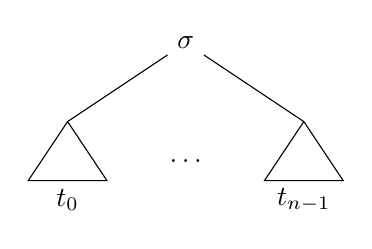
\begin{tikzpicture}
      \node (t1) at (0,-0.5){\(t_0\)};
      \node (t2) at (1.5,0){\(\ldots\)};
      \node (t3) at (3,-0.5){\(t_{n-1}\)};
      \node (s) at (1.5, 1.5){\(\sigma\)};
      
      \draw[-] (0,0.5) -- (.5, -.25) -- (-.5, -.25) -- (0, .5);
      % \draw[-] (1.5,0.5) -- (2, -.25) -- (1, -.25) -- (1.5, .5);
      \draw[-] (3,0.5) -- (3.5, -.25) -- (2.5, -.25) -- (3, .5);

      \draw[-] (s) -- (0,0.5);
      % \draw[-] (s) -- (1.5,0.5);
      \draw[-] (s) -- (3,0.5);
    \end{tikzpicture}
  \end{equation*}
  to the element \((\sigma, (t_0, \ldots, t_{n-1}))\) of \(H_\Sigma(T_\Sigma)\).
  Notice that this is the inverse of tree-tupling (see Remark \ref{rem:treetupling}) so let is be denoted by \(\tau^{-1}\).
  The terminal coalgebra of \(H_\Sigma\) is \((T_\Sigma, \tau^{-1})\).
\end{proposition}

\begin{proof}
  Let \((A, \alpha)\) be a \(H_\Sigma\)-coalgebra and consider the function \(h: A \to T_\Sigma\) that sends \(x \in A\) to the tree \(t_x\) constructed recursively as
  \begin{equation*}
    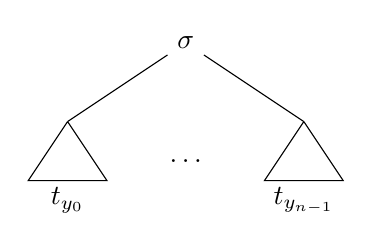
\begin{tikzpicture}
      \node (t1) at (0,-0.5){\(t_{y_0}\)};
      \node (t2) at (1.5,0){\(\ldots\)};
      \node (t3) at (3,-0.5){\(t_{y_{n-1}}\)};
      \node (s) at (1.5, 1.5){\(\sigma\)};
      
      \draw[-] (0,0.5) -- (.5, -.25) -- (-.5, -.25) -- (0, .5);
      % \draw[-] (1.5,0.5) -- (2, -.25) -- (1, -.25) -- (1.5, .5);
      \draw[-] (3,0.5) -- (3.5, -.25) -- (2.5, -.25) -- (3, .5);

      \draw[-] (s) -- (0,0.5);
      % \draw[-] (s) -- (1.5,0.5);
      \draw[-] (s) -- (3,0.5);
    \end{tikzpicture}
  \end{equation*}
  where \(\alpha(x) = (\sigma, y_0, \ldots, y_{n-1})\).
  This is clearly a function such that
  \begin{equation*}
    \begin{tikzcd}[sep=large]
      A \ar[r, "\alpha"] \ar[d, "h"] & H_\Sigma A \ar[d, "H_\Sigma h"] \\
      T_\Sigma \ar[r, "\tau^{-1}"] & H_\Sigma T_\Sigma
    \end{tikzcd}
  \end{equation*}
  commutes i.e. a coalgebra morphism.
  Now let \(g:A \to T_\Sigma\) be another morphism and \(x \in A\) such that \(\alpha(x) = (\sigma, y_0, \ldots, y_{n-1})\) as above.
  Then \(g(x)\) is a tree
  \begin{equation*}
    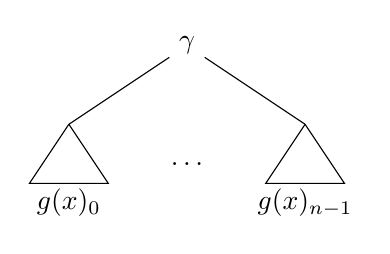
\begin{tikzpicture}
      \node (t1) at (0,-0.5){\(g(x)_0\)};
      \node (t2) at (1.5,0){\(\ldots\)};
      \node (t3) at (3,-0.5){\(g(x)_{n-1}\)};
      \node (s) at (1.5, 1.5){\(\gamma\)};
      
      \draw[-] (0,0.5) -- (.5, -.25) -- (-.5, -.25) -- (0, .5);
      % \draw[-] (1.5,0.5) -- (2, -.25) -- (1, -.25) -- (1.5, .5);
      \draw[-] (3,0.5) -- (3.5, -.25) -- (2.5, -.25) -- (3, .5);

      \draw[-] (s) -- (0,0.5);
      % \draw[-] (s) -- (1.5,0.5);
      \draw[-] (s) -- (3,0.5);
    \end{tikzpicture}
  \end{equation*}
  such that
  \begin{equation*}
    (\gamma, g(x)_0, \ldots, g(x)_{n-1}) = (\tau^{-1} \circ g)(x) = (H_\Sigma g \circ \alpha)(x) = (\sigma, g(y_0), \ldots, g(y_{n-1}))
  \end{equation*}
  so \(\gamma = \sigma\) and \(g(x)_i = g(y_i)\) for \(i < n\) i.e. \(g(x)\) and \(t_x\) have the same root and the \(i\)-th subtree of \(g(x)\) is \(g(y_i)\).
  We can iterate this process to obtain that \(g(x) = t_x\), thus \(g\) must be \(h\), and \((T_\Sigma, \tau^{-1})\) is the terminal coalgebra.
\end{proof}

The necessary condition of Lambeck's Lemma \ref{lemma:lambeck} dualizes as well.

\begin{lemma}[Lambeck's Lemma]
  \label{lemma:colambeck}
  A terminal coalgebra for \(F\), if it exists, is always a fixed point.
\end{lemma}

\begin{proof}
  Dual to that of Lemma \ref{lemma:lambeck}.
\end{proof}

\begin{remark}
  The power-set functor \(\mathcal{P}\) has no terminal coalgebra because it has no fixed point.
  Similarly the functor \(FX = \{0, 1\} \times (\mathbb{P}X)^\Sigma\), which gives non-deterministic automata as coalgebras (see Example \ref{ex:NDA}), does not have a terminal coalgebra.
\end{remark}

Lambeck's Lemma for coalgebras can be interpreted as a generalization of an order-theoretic lemma just as its version for algebras.

\begin{definition}
  Let \((P, \sqsubseteq)\) be a poset and \(f: P \to P\) a monotone function.
  An element \(x \in P\) is a \textbf{post-fixed point} if \(x \sqsubseteq f(x)\).
\end{definition}

\begin{lemma}
  Given a poset \((P, \sqsubseteq)\) and a monotone function \(f: P \to P\) let \(A = \{x \in P : x \sqsubseteq f(x)\}\) be the set of post-fixed points of \(f\).
  If \(\overline{a}\) is the join of \(A\) then \(\overline{a}\) is the biggest fixed-point of \(f\).
\end{lemma}

\begin{proof}
  A classical proof can be obtained by dualizing the one of Lemma \ref{lemma:order_theory}.
  Otherwise it follows from Lambeck's Lemma \ref{lemma:colambeck} once one notices that post-fixed points for \(f\) are just \(f\)-coalgebras.
\end{proof}

The Knaster-Tarski Theorem \ref{teo:knaster_tarski} obviously follows from this version of the lemma as well since the hypothesis guarantee the existence of the join of \(A\).

\begin{remark}
  By Theorem \ref{teo:set_lambeck_converse} and Lambeck's Lemma we have that, for functors over \(\Set\), the existence of a terminal coalgebra implies the existence of an initial algebra.
  The converse is false since, as it was found in \cite[Example 3.14]{Adamek-2016} by Adámek, Koubek and Palm, there are two set functors that coincide on all objects (but not all morphisms) such that one has a terminal coalgebra and the other one does not (we shall see this in Section [TO DO]).
  Thus the existence of a terminal coalgebra, even for set functors, is a more complicated matter than the existence of an initial algebra.
\end{remark}

\section{Corecursion and Bisimulation}

We strive now to dualize what we have seen about recursion and induction in Section \ref{sec:recursion_and_induction}.
Recursion is dualized straightforwardly but we don't do the same for induction.
Instead of coinduction we will discuss bisimulation, a concept that has many applications, for instance, in computer science and modal logic.

\begin{definition}
  Let \(F\) be an endofuctor over some category \(\A\) with a terminal coalgebra \(\nu F\).
  A morphism \(f: A \to \nu F\) of \(\A\) is \textbf{corecursively specified} \marginnote{corecursively specified morphism} if there is a coalgebra structure \(\alpha : A \to FA\) on \(A\) that makes \(f\) into a morphism of coalgebras (actually \(f\) is unique since \(\nu F\) is terminal).
\end{definition}

\begin{example}
  \label{ex:corecursive-specification-of-addition}
  As for Example \ref{ex:terminalcoalgebra1} the terminal coalgebra for \(FX = X + 1\) over \(\Set\) is \((\mathbb{N}^\top, \tau)\).
  We shall see that the function \(\textsf{add} : \mathbb{N}^\top \times \mathbb{N}^\top \to \mathbb{N}^\top\) defined as addition of natural numbers extended by \(x + \infty = \infty, \infty + x = \infty\) and \(\infty + \infty = \infty\) is corecursively specified.
  In order to do so we need a coalgebra structure on \(\mathbb{N}^\top \times \mathbb{N}^\top\) that induces \(\textsf{add}\) as the unique coalgebra morphism to \(\mathbb{N}^\top\).
  Consider then the coalgebra given by the following structure \(\alpha: \mathbb{N}^\top \times \mathbb{N}^\top \to \mathbb{N}^\top \times \mathbb{N}^\top + 1\):
  \begin{itemize}
  \item[1.] the only terminal state is \((0, 0)\);
  \item[2.] if \((x, y)\) is not terminal then we set
    \begin{equation*}
      \alpha(x, y) =
      \begin{cases}
        (0, \tau(y)) & \text{if } x = 0\\
        (\tau(x), y) & \text{if } x \neq 0
      \end{cases}.
    \end{equation*}
  \end{itemize}
  Now let \(b_A : \mathbb{N}^\top \times \mathbb{N}^\top \to \mathbb{N}^\top\) be the unique morphism to the terminal coalgebra and notice that a state \((x, y)\), under iterated applications of \(\alpha\), either reaches \((0, 0)\) in \(x + y\) steps or generates an infinite sequence exactly when \(x = \infty\) or \(y = \infty\).
  Thus we have that \(b_A = \textsf{add}\).
\end{example}

\begin{example}
  Consider the functor \(FX = \Sigma \times X\) over \(\Set\) with \(\Sigma\) a fixed set of outputs.
  We know from Example \ref{ex:transition_systems_with_outputs} that the terminal coalgebra for \(F\) is \(\Sigma^\infty\), the set of \(\Sigma\)-streams, with structure given by \(\tau = \intoprod{\head}{\tail}\).

  A single stream can be identified with the function \(f : 1 \to \Sigma^\infty\) that picks it so we say that a stream is corecursively specified if its \(f : 1 \to \Sigma^\infty\) is corecursively specified.
  Coalgebra structures on \(1\) are functions \(\alpha: 1 \to \Sigma \times 1\) so the only corecursively specifiable streams are the constant ones.

  Other kinds of streams can be corecursively specified as well.
  For example consider the set \(2\) with the coalgebra structure given by \(\alpha : 2 \to \Sigma \times 2\) defined by \(\alpha(0) = (x, 1)\) and \(\alpha(1) = (y, 0)\) for \(x, y \in \Sigma\).
  Graphically this coalgebra can be represented as
  \begin{equation*}
    \begin{tikzcd}[sep = large]
      0 \ar[r, bend left, "x"] & 1 \ar[l, bend left, "y"]
    \end{tikzcd}.
  \end{equation*}
  Since \(\Sigma^\omega\) is the terminal coalgebra there is a unique \(h : 2 \to \Sigma^\omega\) such that
  \begin{equation*}
    \intoprod{\head}{\tail} \circ h = (\id \times h) \circ \alpha
  \end{equation*}
  from which we obtain the following relations
  \begin{itemize}
  \item[1.] \(\head(h(0)) = \alpha(0) = x\) and \(\head(h(1)) = \alpha(1) = y\);
  \item[2.] \(\tail(h(0)) = h(\alpha(0)) = h(1)\) and \(\tail(h(1)) = h(\alpha(1)) = h(0)\);
  \end{itemize}
  and thus we must have
  \begin{equation*}
    h(0) = (x, y, x, y, \ldots) \text{ and } h(1) = (y, x, y, x, \ldots).
  \end{equation*}
  So alternating streams can also be corecursively constructed.

  Finally we look at an example of a corecursively specifiable function on streams: the \(\textsf{zip}\) function.
  Given two streams \(x = (x_0, x_1, \ldots), y = (y_0, y_1, \ldots)\) we define a new stream
  \begin{equation*}
    \textsf{zip}(x, y) = (x_0, y_0, x_1, y_1, \ldots).
  \end{equation*}
  We give \(\Sigma^\omega \times \Sigma^\omega\) a coalgebra structure \(\alpha = \intoprod{\alpha_\head}{\alpha_\tail}\) by defining
  \fundef{\alpha_\head}{\Sigma^\omega \times \Sigma^\omega}{\Sigma}{(x, y)}{\head(x)}
  \fundef{\alpha_\tail}{\Sigma^\omega \times \Sigma^\omega}{\Sigma^\omega \times \Sigma^\omega}{(x, y)}{(y, \tail(x))}
  and notice that the following squares commute
  \begin{equation*}
    \begin{tikzcd}[sep = large]
      \Sigma^\omega \times \Sigma^\omega \ar[r, "\alpha_\head"] \ar[d, "\textsf{zip}"] & \Sigma \ar[d, "\id"] \\
      \Sigma^\omega \ar[r, "\head"] & \Sigma
    \end{tikzcd}\quad
    \begin{tikzcd}[sep = large]
      \Sigma^\omega \times \Sigma^\omega \ar[r, "\alpha_\tail"] \ar[d, "\textsf{zip}"] & \Sigma^\omega \times \Sigma^\omega \ar[d, "\textsf{zip}"] \\
      \Sigma^\omega \ar[r, "\alpha_\tail"] & \Sigma^\omega
    \end{tikzcd}.
  \end{equation*}
  Thus we have that \(\textsf{zip}\) is corecursively specified.
\end{example}

\begin{theorem}[Primitive Corecursion]
  \label{th:primitive_corecursion}
  Assume the category \(\A\) has finitite coproducts and \(F\) is an endofuctor on \(\A\) with a terminal coalgebra.
  Then for every \(\alpha : X \to F(X + \nu F)\) there is a unique \(h : X \to \nu F\) such that the following square commutes
  \begin{equation*}
    \begin{tikzcd}[sep = large]
      X \ar[r, "\alpha"] \ar[d, "h"] & F(X + \nu F) \ar[d, "F\outofcoprod{h}{\id_{\nu F}}"]\\
      \nu F \ar[r, "\tau"] & F(\nu F)
    \end{tikzcd}.
  \end{equation*}
\end{theorem}

\begin{proof}
  Dual to that of Theorem \ref{teo:primitive_recursion}.
\end{proof}

\begin{definition}
  \label{def:bisimulation}
  Let \((A, \alpha)\) and \((B, \beta)\) be two \(F\)-coalgebras for a functor \(F\) over a category \(\A\) with binary products.
  A \textbf{bisimulation} \marginnote{bisimulation} between them is a relation
  \begin{equation*}
    \intoprod{r_A}{r_B} : R \rightarrowtail A \times B
  \end{equation*}
  together with a coalgebra structure \(\rho\) on \(R\) that makes \(r_A\) and \(r_B\) into morphisms of coalgebras i.e. the following squares
  \begin{equation*}
    \begin{tikzcd}[sep = large]
      R \ar[r, "\rho"] \ar[d, "r_A"] & FR \ar[d, "Fr_A"] \\
      A \ar[r, "\alpha"] & FA
    \end{tikzcd}\quad
    \begin{tikzcd}[sep = large]
      R \ar[r, "\rho"] \ar[d, "r_B"] & FR \ar[d, "Fr_B"] \\
      B \ar[r, "\beta"] & FB
    \end{tikzcd}
  \end{equation*}
  commute.
  When the two coalgebras are the same, say \((A, \alpha)\), we speak of a bisimulation on \((A, \alpha)\).
\end{definition}

\begin{remark}
  In the above definition by saying that \(\intoprod{r_A}{r_B}\) is a relation we simply mean that it is a monomorphism i.e. it represents a subobject of \(A \times B\).
%   Moreover we recall that \(\intoprod{r_A}{r_B}\) is monic if and only if both \(r_A\) and \(r_B\) are.
\end{remark}

The intuition behind the definition is that two states in two different coalgebras related by a bisimulation have the same behaviour.
An example should clarify the matter.
\begin{example}
  Consider a pair of systems with termination (see Example \ref{ex:systems-with-termination})
  \begin{equation*}
    \alpha: A \to A + 1 \text{ and } \beta: B \to B + 1.
  \end{equation*}
  Then a bisimulation between them is a relation \(R \subseteq A \times B\), with coalgebra structure \(\rho\) on \(R\), such that if \(x R y\) then
  \begin{itemize}
  \item[1.] \(x\) is terminal if and only if \(y\) is terminal;
  \item[2.] if \(x, y\) are not terminal and \(x', y'\) are their respective next states then \(x' R y'\).
  \end{itemize}
  Indeed by the definition of bisimulation we have that the following squares in \(\Set\) commute.
  \begin{equation}
    \label{dia:fooooo}
    \begin{tikzcd}[sep = large]
      R \ar[r, "\rho"] \ar[d, "r_A"] & R + 1 \ar[d, "r_A + \id_1"] \\
      A \ar[r, "\alpha"] & A + 1
    \end{tikzcd}\quad
    \begin{tikzcd}[sep = large]
      R \ar[r, "\rho"] \ar[d, "r_B"] & R + 1 \ar[d, "r_B + \id_1"] \\
      B \ar[r, "\beta"] & B + 1
    \end{tikzcd}
  \end{equation}
  Recall moreover that \(x R y\) means that \((x, y) \in R\) so:
  \begin{itemize}
  \item[a.] since \(r_A\) is a coalgebra morphism we have \((x, y)\) is terminal in \(R\) if and only if \(x\) is terminal in \(A\) and, similarly using \(r_B\), \((x, y)\) is terminal in \(R\) if and only if \(y\) is terminal in \(B\); thus we obtain \(1\) above;
  \item[b.] if \(x, y\) are not terminal then, since \(r_A, r_B\) are morphisms, we obtain
    \begin{equation*}
      (r_A \circ \rho)(x, y) = (\alpha \circ r_A)(x, y) = \alpha(x) = x',
    \end{equation*}
    \begin{equation*}
      (r_B \circ \rho)(x, y) = (\beta \circ r_B)(x, y) = \beta(y) = y'.
    \end{equation*}
    Thus \(\rho(x, y) = (x', y')\) and we have 2.
  \end{itemize}

  On the other hand if 1 and 2 hold we can make \(R\) into a coalgebra \(\rho : R \to R + 1\) such that \(\rho(x, y) = (x', y')\) if \(x\) is not terminal and \(\rho(x, y) = *\) in the right summand if \(x\) is terminal.
  The projections \(r_A, r_B\) are clearly make the squares \ref{dia:fooooo} commute since they preserve next-states and preserve and reflect terminal ones.

  In virtue of conditions 1 and 2 we obtain immediately that the unique morphisms \(b_A : A \to \mathbb{N}^\top, b_B : B \to \mathbb{N}^\bot\) into the terminal coalgebra are such that, for every bisimulation \(R\), \(x R y\) implies \(b_A(x) = b_B(y)\) which formalizes the idea of bisimulations ``linking'' states with the same behaviour.
\end{example}

\begin{definition}
  The \textbf{diagonal subobject} \marginnote{diagonal subobject} \(\Delta_A\) of \(A \times A\) is the one represented by \(\intoprod{\id_A}{\id_A}: A \rightarrowtail A \times A\).
\end{definition}

\begin{remark}
  The diagonal subobject \(\Delta_A\) is always a bisimulation on any coalgebra \((A, \alpha)\).
  A bisibulation not contained in \(\Delta_A\) is a \textbf{proper bisimulation}\marginnote{proper bisimulation}.
  Moreover notice that a relation \(\intoprod{r_1}{r_2}: R \rightarrowtail A \times A\) is proper if \(r_1 = r_2\).
\end{remark}

Finally we can state and prove the coinduction principle.

\begin{theorem}[Coinduction Principle]
  Let \(F\) be an endofunctor with a terminal coalgebra \(\nu F\).
  There are no proper bisimulations on \(\nu F\).
\end{theorem}

\begin{proof}
  Let \(r = \intoprod{r_1}{r_2}: R \rightarrowtail \nu F \times \nu F\) be a bisimulation i.e. \(R\) has a coalgebra structure such that \(r_1\) and \(r_2\) are coalgebra morphisms.
  By terminality of \(\nu F\) we must have \(r_1 = r_2\) and thus the bisimulation is proper.
\end{proof}

The coinduction principle ties into our interpretation of bisimulations linking states that have the same behaviour by saying that no two states in the terminal coalgebra have the same behaviour.
Terminal coalgebras we can thus think of as containing all possible behaviours and nothing more.

\printbibliography
\end{document}
